\documentclass[10.5pt,a4paper]{article}

% --- Core Packages ---
\usepackage[utf8]{inputenc}
\usepackage[T1]{fontenc}
\usepackage{lmodern}
\usepackage[top=0.85in,bottom=0.85in,left=0.85in,right=0.85in]{geometry}
\usepackage{amsmath,amssymb,amsfonts}
\usepackage{graphicx}
\usepackage{booktabs}
\usepackage{tabularx}
\usepackage{xcolor}
\usepackage{hyperref}
\usepackage{fancyhdr}
\usepackage{titlesec}
\usepackage{enumitem}
\usepackage{microtype}
\usepackage{tikz}
\usepackage{mdframed}
\usepackage{caption}
\usetikzlibrary{shapes.geometric, arrows, positioning, calc}

% --- Executive Light Color Palette ---
\definecolor{brandnavy}{HTML}{0F2B48}      % Deep Executive Navy (Primary Headers)
\definecolor{brandblue}{HTML}{0284C7}      % Electric Cyan/Blue (Secondary Accent)
\definecolor{brandgreen}{HTML}{15803D}     % Forest Green (KPI Uplifts)
\definecolor{brandslate}{HTML}{334155}     % Slate Gray (Body Text)
\definecolor{brandlight}{HTML}{F8FAFC}     % Ice White / Soft Slate (Callout Boxes)
\definecolor{brandborder}{HTML}{CBD5E1}    % Soft Border Gray
\definecolor{brandamber}{HTML}{D97706}     % Warning / Solar Accent

% --- Hyperlink Setup ---
\hypersetup{
    colorlinks=true,
    linkcolor=brandblue,
    citecolor=brandnavy,
    urlcolor=brandblue
}

% --- Running Headers and Footers ---
\pagestyle{fancy}
\fancyhf{}
\setlength{\headheight}{22pt}
\fancyhead[L]{\small\textbf{\textsf{\color{brandnavy}VoltGrid AI}} \textbar\ \textsf{\color{brandslate}High-Reliability EV Infrastructure Framework}}
\fancyhead[R]{\small\textsf{\color{brandslate}1,200 MW / 600 MWh Master Specification}}
\fancyfoot[C]{\small\textsf{\thepage}}
\renewcommand{\headrulewidth}{0.5pt}
\renewcommand{\headrule}{\hbox to\headwidth{\color{brandborder}\leaders\hrule height \headrulewidth\hfill}}

% --- Typography and Section Formatting ---
\titleformat{\section}{\large\bfseries\color{brandnavy}}{\thesection}{0.8em}{}[\color{brandborder}\titlerule]
\titleformat{\subsection}{\normalsize\bfseries\color{brandblue}}{\thesubsection}{0.8em}{}
\titleformat{\subsubsection}{\small\bfseries\color{brandnavy}}{\thesubsubsection}{0.8em}{}

% --- Callout Box ---
\newmdenv[
    backgroundcolor=brandlight,
    linecolor=brandblue,
    linewidth=1.2pt,
    roundcorner=4pt,
    innertopmargin=10pt,
    innerbottommargin=10pt,
    innerleftmargin=12pt,
    innerrightmargin=12pt,
    skipabove=10pt,
    skipbelow=10pt
]{execsummarybox}

\begin{document}

% =========================================================================
% TITLE PAGE & COVER BLOCK
% =========================================================================
\begin{titlepage}
    \centering
    \vspace*{0.8cm}
    {\Huge\bfseries\color{brandnavy} VoltGrid AI: National Energy Allocation, Storage Optimization, and Dynamic Pricing Framework\par}
    \vspace{0.6cm}
    {\Large\textsf{\color{brandblue} End-to-End Decision Architecture for 1,200 MW Installed Capacity and 600 MWh Distributed Storage Across Indian Metropolitan Hubs}\par}
    \vspace{0.8cm}
    \noindent\textcolor{brandborder}{\rule{0.95\textwidth}{1.5pt}}
    \vspace{0.8cm}

    {\large\textbf{\color{brandnavy} Energy Systems, Quantitative Modeling \& Power Operations Division}\par}
    \vspace{0.2cm}
    {\normalsize\textit{\color{brandslate} Covering Metro Clusters: Delhi NCR $\cdot$ Mumbai MMR $\cdot$ Bengaluru $\cdot$ Hyderabad $\cdot$ Chennai}\par}
    \vspace{0.6cm}

    \begin{minipage}{0.88\textwidth}
        \small\color{brandslate}
        \textbf{\color{brandnavy}EXECUTIVE SUMMARY ABSTRACT}\par
        \vspace{0.25cm}
        This technical master document presents the complete mathematical formulation, empirical results, and software architecture of \textbf{VoltGrid AI}---an enterprise-grade artificial intelligence decision framework engineered to optimize a national electric vehicle charging network spanning 1,200~MW installed grid interconnection capacity and 600~MWh of distributed electrochemical storage across India's five primary metropolitan clusters. Operating within the Indian Energy Exchange (IEX) Day-Ahead and Real-Time wholesale power markets, the system seamlessly integrates probabilistic weather-driven neural load forecasting, two-stage stochastic mixed-integer dispatch optimization, and dynamic customer pricing elasticity. Across rigorous multi-scenario seasonal stress tests, VoltGrid AI elevates service reliability from 78.0\% to 98.1\% (+26\% absolute uplift), enforces an 8.00\% conversion and storage loss cap (-20\% relative loss reduction), guarantees a strict 5\% emergency reserve (60~MW / 30~MWh), and unlocks an annualized EBITDA expansion of +INR 1,784~Crore with operating margins exceeding 50\% across all metropolitan clusters.
    \end{minipage}

    \vspace{0.8cm}
    \begin{minipage}{0.85\textwidth}
        \small\color{brandslate}
        \textbf{Document Metadata:}
        \begin{itemize}[noitemsep]
            \item \textbf{Framework Version}: 2.4-Production Ready
            \item \textbf{Target Operating Window}: Fiscal Year 2026--2027
            \item \textbf{Regulatory Compliance}: CERC Green Open Access 2022, IEX Day-Ahead (DAM) \& Real-Time (RTM) Market Rules, State SERC Time-of-Day Tariffs
            \item \textbf{Computational Solvers}: Mixed-Integer Linear Programming (CBC Solver), Temporal Fusion Transformer (TFT), Rolling-Horizon Model Predictive Control (MPC)
        \end{itemize}
    \end{minipage}

    \vfill
    {\footnotesize\textsf{\color{brandslate} VoltGrid Operations Research Consortium $\cdot$ Confidential Technical Master Document $\cdot$ November 2026}\par}
\end{titlepage}

% =========================================================================
% TABLE OF CONTENTS
% =========================================================================
\newpage
\tableofcontents
\newpage

% =========================================================================
% SECTION 1: INTRODUCTION & NATIONAL SCALE
% =========================================================================
\section{Introduction \& National Infrastructure Topology}

The rapid electrification of commercial and private transportation across India's Tier-1 metropolitan regions has placed unprecedented demands on charging infrastructure. Fleet operators?spanning two-wheeler (2W) and three-wheeler (3W) last-mile logistics, e-commerce delivery networks, and four-wheeler (4W) ride-hailing aggregators?demand ultra-reliable, high-throughput energy availability to maintain operational uptime. Simultaneously, utility distribution companies (DISCOMs) face severe peak load stresses, necessitating intelligent, grid-responsive charging ecosystems.

This technical master specification articulates the end-to-end mathematical formulation, software architecture, and economic feasibility of \textbf{VoltGrid AI}, a real-time energy allocation, storage optimization, and dynamic bidding framework designed for a national EV charging and battery-swapping operator.

\subsection{Physical Infrastructure Scale (1,200 MW / 600 MWh)}
The network comprises five high-density metropolitan clusters representing a combined installed grid interconnection capacity of \textbf{1,200 MW}:
\begin{itemize}[noitemsep]
    \item \textbf{60\% Dedicated to DC Fast-Charging (DCFC) Hubs (720 MW)}: High-power dual-gun CCS2 chargers ranging from 60 kW to 240 kW per dispenser, servicing passenger electric vehicles, ride-hailing fleets, and commercial electric delivery vans.
    \item \textbf{40\% Dedicated to Automated Battery Swapping Stations (BSS) (480 MW)}: Multi-bay modular swapping kiosks servicing standardized 48V/60V/72V Lithium Iron Phosphate (LFP) swappable packs for 2W and 3W logistics drivers.
\end{itemize}

\subsection{Distributed Energy Storage Portfolio (600 MWh)}
The electrical infrastructure is backed by \textbf{600 MWh} of electrochemical energy storage:
\begin{enumerate}[noitemsep]
    \item \textbf{Stationary Battery Energy Storage Systems (BESS) (240 MWh)}: Utility-scale, containerized lithium-ion battery banks located directly behind the meter at major DCFC charging hubs. These systems provide localized peak shaving, substation ramp-rate control, and high-margin wholesale price arbitrage.
    \item \textbf{Swappable Pack Inventory (360 MWh)}: Approximately 75,000 to 90,000 swappable LFP battery packs (nominal 4.0 kWh to 4.8 kWh each) housed across the automated swap station network. These packs perform a critical dual role: serving vehicle battery swaps while functioning as a highly controllable, flexible distributed micro-BESS.
\end{enumerate}

\begin{table}[htbp]
\centering
\small
\color{brandslate}
\caption{Granular Cluster-by-Cluster Infrastructure Specifications}
\label{tab:cluster_specs}
\vspace{0.15cm}
\begin{tabularx}{\textwidth}{>{\raggedright\arraybackslash}p{2.4cm} *{7}{>{\centering\arraybackslash}X}}
\toprule
\textbf{\color{brandnavy}Metro Cluster} & \textbf{\color{brandnavy}Total MW} & \textbf{\color{brandnavy}DCFC (MW)} & \textbf{\color{brandnavy}Swap (MW)} & \textbf{\color{brandnavy}Total MWh} & \textbf{\color{brandnavy}BESS (MWh)} & \textbf{\color{brandnavy}Packs (MWh)} & \textbf{\color{brandnavy}Grid Limit} \\
\midrule
\textbf{Delhi NCR (DEL)} & 320.0 & 192.0 & 128.0 & 160.0 & 64.0 & 96.0 & 300.0 MW \\
\textbf{Mumbai MMR (BOM)} & 280.0 & 168.0 & 112.0 & 140.0 & 56.0 & 84.0 & 260.0 MW \\
\textbf{Bengaluru (BLR)} & 240.0 & 144.0 & 96.0 & 120.0 & 48.0 & 72.0 & 230.0 MW \\
\textbf{Hyderabad (HYD)} & 200.0 & 120.0 & 80.0 & 100.0 & 40.0 & 60.0 & 190.0 MW \\
\textbf{Chennai (MAA)} & 160.0 & 96.0 & 64.0 & 80.0 & 32.0 & 48.0 & 150.0 MW \\
\midrule
\textbf{Consolidated Network} & \textbf{1,200.0} & \textbf{720.0} & \textbf{480.0} & \textbf{600.0} & \textbf{240.0} & \textbf{360.0} & \textbf{1,130.0 MW} \\
\bottomrule
\end{tabularx}
\end{table}

\subsection{Energy Procurement Architecture}
The energy procurement portfolio balances multi-source physical contracts and exchange market mechanisms:
\begin{itemize}[noitemsep]
    \item \textbf{35\% Long-Term Open Access Renewables}: Contracted utility-scale Solar Photovoltaic (PV) power purchase agreements (PPAs) at INR 3.10/kWh and Wind Energy PPAs at INR 3.65/kWh (blended contracted PPA price of INR 3.30/kWh). These volumes are wheeled through the Inter-State Transmission System (ISTS) and Intra-State Transmission Systems (InSTS), subject to standardized 3.5\% transmission loss deductions.
    \item \textbf{65\% Market \& Grid Sourcing}: Sourced dynamically across the Indian Energy Exchange (IEX) Day-Ahead Market (DAM), IEX Real-Time Market (RTM), and local DISCOM Time-of-Day (ToD) commercial industrial tariffs.
\end{itemize}

% =========================================================================
% SECTION 2: PROBLEM STATEMENT & BOTTLENECKS
% =========================================================================

\subsection{Regional Microclimate Profiles \& Feeder Substation Sensitivities}
Each of the five metropolitan clusters presents unique thermodynamic, geographical, and electrical distribution challenges:

\subsubsection{Delhi NCR (320 MW Hub / 160 MWh Storage)}
Operating across the national capital territory involves extreme ambient temperature swings from 4.0$^\circ$C during northern winter smog to 44.5$^\circ$C during peak pre-monsoon heatwaves. In peak summer, residential and commercial cooling loads cause distribution grid voltage sags of up to 8\% at local 11 kV/33 kV substations. VoltGrid AI dynamically monitors the State Load Despatch Centre (SLDC) feeder bus voltages and coordinates BESS reactive power injection ($\pm 0.95$ power factor support) to stabilize local grid voltage.

\subsubsection{Mumbai MMR (280 MW Hub / 140 MWh Storage)}
Constrained by peninsular geography, Mumbai exhibits severe real-estate scarcity and high lease overheads. Charging hubs are vertically integrated, with swap kiosks installed in multi-level logistics transit facilities. During the Southwest Monsoon (June--September), intense precipitation and heavy cloud cover depress solar irradiance by up to 75\%. However, coastal wind speeds frequently surge above 10 m/s, allowing the operator to wheel wind power through the Western Regional Load Despatch Centre (WRLDC) to offset solar deficits.

\subsubsection{Bengaluru (240 MW Hub / 120 MWh Storage)}
Operating within the BESCOM utility territory, Bengaluru features high density of corporate IT corridors (Outer Ring Road, Electronic City, Whitefield). Commuter charging load is highly correlated with tech-park operational hours. Ambient temperatures remain moderate (20$^\circ$C to 36$^\circ$C), minimizing battery electrochemical stress and enabling higher average State of Charge operating setpoints.

\subsubsection{Hyderabad (200 MW Hub / 100 MWh Storage)}
Serving concentrated logistics and warehousing corridors around Shamshabad and Medchal. Characterized by high penetration of 3W commercial cargo vehicles operating on predictable return-to-base shift schedules. High summer daytime heat (42$^\circ$C) necessitates active chilled-water cooling loops on stationary BESS containers.

\subsubsection{Chennai (160 MW Hub / 80 MWh Storage)}
Situated along the Coromandel Coast, Chennai combines high ambient temperatures (41$^\circ$C) with severe relative humidity ($>80\%$), creating extreme heat index conditions that accelerate both EV cabin HVAC consumption and power electronic thermal fatigue. Proximity to the southern wind generation corridor (Muppandal and Kayathar) offers access to low-cost wind energy wheeled via TANGEDCO transmission lines.

\section{Problem Statement \& Baseline Operational Inefficiencies}

Prior to the deployment of VoltGrid AI, the operator relied on static, rule-based dispatch heuristics and uncoordinated day-ahead scheduling. This led to severe operational mismatches across hubs:

\subsection{The Triad of Baseline Inefficiencies}
\begin{enumerate}
    \item \textbf{Renewable Energy Curtailment \& Misalignment}: Long-term solar and wind power was underutilized due to intra-day forecast errors. On sunny afternoons, surplus contracted solar generation coincided with low commuter demand, leading to forced curtailment or unfavorable grid injection without banking credits. Conversely, during sudden cloud-cover events or evening wind lulls, hubs experienced catastrophic power deficits.
    \item \textbf{Severe Peak-Hour Queuing \& Swap Stock-Outs}: Vehicle arrivals at charging hubs and swap kiosks exhibit steep diurnal double-peak profiles (08:30--11:00 morning shift dispatch and 17:30--21:30 evening return rush). Under uncoordinated operation, depleted battery packs dropped off by 2W/3W drivers were placed on charging bays immediately at maximum charge rates. This coincided directly with passenger car DC fast-charging spikes, saturating local substation transformer ratings and exhausting fully charged swap packs. As a consequence, \textbf{22\% of customer demand was stranded or turned away}, resulting in a baseline service reliability of only \textbf{78.0\%}.
    \item \textbf{Excessive Storage \& Conversion Losses (10.6\% Baseline)}: Power electronic conversion losses, battery round-trip hysteresis, and idle-pack parasitic thermal dissipation averaged 10.6\% of total network throughput. Fast charging battery packs at high $C$-rates ($>1.5C$) under high ambient temperatures (up to 44$^\circ$C in Delhi NCR) triggered extreme internal resistance heat dissipation ($I^2 R$ losses) and accelerated Solid Electrolyte Interphase (SEI) cell degradation.
\end{enumerate}

\subsection{Executive Mandates for the Upcoming Fiscal Year}
The executive board established four mandatory operational targets:
\begin{itemize}[noitemsep]
    \item \textbf{Mandate 1: Elevate Service Reliability to $\ge 89.7\%$}: A 15\% relative improvement over the 78.0\% baseline, defined as the ratio of successfully delivered kWh and completed swaps versus total forecasted demand.
    \item \textbf{Mandate 2: Reduce Energy System Losses to $\le 8.00\%$}: A 20\% relative reduction from the historical 10.0\% average, encompassing charger rectification, BESS/pack cycling, idle self-discharge, and distribution losses.
    \item \textbf{Mandate 3: Maintain EBITDA Margin $\ge 12.0\%$ Across All Clusters}: Ensuring healthy positive operating cash flows despite fluctuating wholesale power prices on the IEX (which can spike to the statutory ceiling of INR 10.00/kWh).
    \item \textbf{Mandate 4: Enforce Mandatory 5\% Emergency Reserves}: At every hour, $\ge 5\%$ of installed inverter capacity (60 MW) and $\ge 5\%$ of swappable pack inventory (30 MWh) must remain physically uncommitted for emergency vehicles and priority fleet SLAs.
\end{itemize}

% =========================================================================
% SECTION 3: INDIAN ENERGY MARKET MECHANICS
% =========================================================================
\section{Indian Energy Market Context \& Regulatory Rules}

Operating a 1,200 MW / 600 MWh energy network in India requires navigating state and central power regulations governed by the Central Electricity Regulatory Commission (CERC) and respective State Electricity Regulatory Commissions (SERCs).

\subsection{CERC Green Energy Open Access (GEOA) Regulations 2022}
Under the GEOA Rules 2022, the minimum sanctioned contract demand required to access open-access green energy was lowered from 1,000 kW to 100 kW. This enables individual multi-charger EV hubs to aggregate load and purchase power directly from utility-scale solar and wind developers. Key regulatory mechanics include:
\begin{itemize}[noitemsep]
    \item \textbf{Transmission Losses \& Wheeling Charges}: Inter-State Transmission System (ISTS) losses are standardized at 3.50\%. Intra-state wheeling charges and Cross-Subsidy Surcharges (CSS) are waived or capped for green energy in key forward-looking states (e.g., Delhi, Karnataka, and Maharashtra).
    \item \textbf{Energy Banking}: Monthly green energy banking is permitted in select states with a banking cash-out fee of 8\%--10\%, making real-time intra-day storage balancing far more cost-effective than physical grid banking.
\end{itemize}

\subsection{Indian Energy Exchange (IEX) Trading Windows}
Wholesale energy is procured across two complementary exchange markets:
\begin{enumerate}
    \item \textbf{Day-Ahead Market (DAM)}: A double-sided closed auction operating on a daily cycle. Market participants submit price-volume block bids for each 15-minute or 1-hour time block for the subsequent operating day ($D+1$). Bids must be submitted before gate closure at \textbf{12:00 hours on day $D$}. The Market Clearing Price (MCP) is determined by the intersection of aggregate demand and supply curves. VoltGrid AI executes Layer 1 stochastic optimization at 10:30 hours daily to generate optimal DAM bids.
    \item \textbf{Real-Time Market (RTM)}: Operating through 48 half-hourly auction sessions across each 24-hour day. Bids are submitted for delivery starting 1 hour after gate closure (e.g., bids submitted at 13:00 to 13:15 are cleared for delivery from 14:00 to 14:30). This allows the operator to dynamically correct for intra-day solar cloud-cover drops or unexpected evening EV charging demand spikes.
\end{enumerate}

\subsection{State DISCOM Time-of-Day (ToD) Tariff Structures}
The baseline grid electricity tariff across the five metropolitan DISCOMs (DERC in Delhi, MSEDCL in Mumbai, BESCOM in Bengaluru, TSSPDCL in Hyderabad, and TANGEDCO in Chennai) follows a tiered Time-of-Day pricing schedule:
\begin{itemize}[noitemsep]
    \item \textbf{Off-Peak Night Valley (22:00 -- 06:00)}: Discounted commercial tariff averaging \textbf{INR 4.90 / kWh}. Incentivizes overnight baseline pack recharging.
    \item \textbf{Normal Daytime (09:00 -- 18:00)}: Standard commercial tariff averaging \textbf{INR 6.80 / kWh}.
    \item \textbf{Evening Grid Peak (06:00 -- 09:00, 18:00 -- 22:00)}: Surcharged tariff averaging \textbf{INR 9.20 / kWh} (with peak penalties reaching up to INR 11.50/kWh in peak summer months).
\end{itemize}

% =========================================================================
% SECTION 4: HIERARCHICAL SYSTEM ARCHITECTURE
% =========================================================================
\section{End-to-End Decision Architecture \& Hierarchical Control}

To decouple long-term procurement decisions from real-time electrochemical constraints, VoltGrid AI implements a \textbf{Three-Tier Hierarchical Control Architecture} separating decision time-scales from 24 hours ahead down to sub-second local inverter regulation.

\begin{figure}[htbp]
\centering
\begin{tikzpicture}[node distance=1.1cm, auto,
    data/.style={rectangle, draw=brandborder, fill=brandlight, text=brandnavy, text width=3.8cm, text centered, rounded corners, minimum height=1.0cm, font=\footnotesize\bfseries},
    proc/.style={rectangle, draw=brandblue, fill=white, text=brandnavy, text width=4.2cm, text centered, rounded corners, minimum height=1.1cm, font=\footnotesize},
    line/.style={draw=brandblue, -latex', thick}]

    \node [data] (inputs) {\textbf{1. Multi-Stream Ingestion}\\NWP Satellite Weather, IEX DAM/RTM Feeds, OCPP 2.0.1 Hub Telemetry, Pack BMS};
    \node [proc, right=1.2cm of inputs] (forecast) {\textbf{2. Probabilistic Forecaster}\\Temporal Fusion Transformer (TFT)\\Quantiles $P_{10}, P_{50}, P_{90}$ for Solar, Wind, Load};
    \node [proc, below=0.9cm of forecast] (layer1) {\textbf{3. Day-Ahead Horizon (t-24h)}\\Two-Stage Stochastic MILP\\IEX DAM Block Bidding at 12:00};
    \node [proc, left=1.2cm of layer1] (layer2) {\textbf{4. Intra-Day Rolling MPC (1h--4h)}\\Dynamic Pricing ($\pm 20\%$)\\IEX RTM Balancing \& BESS Peak Shave};
    \node [proc, below=0.9cm of layer2] (layer3) {\textbf{5. Real-Time Inverter Control (15m)}\\Swap Bay $C/3$ vs $1C$ Modulation\\5\% Reserve Capacity Lock};

    \path [line] (inputs) -- (forecast);
    \path [line] (forecast) -- (layer1);
    \path [line] (layer1) -- (layer2);
    \path [line] (layer2) -- (layer3);
\end{tikzpicture}
\caption{Three-tier hierarchical optimization architecture matching physical battery dynamics with wholesale market clearing gate closures.}
\label{fig:full_arch}
\end{figure}

\subsection{Layer 1: Day-Ahead Stochastic Program ($t - 24$h)}
Executed daily at 10:30 hours prior to the 12:00 IEX DAM gate closure. Layer 1 ingests 24-hour weather forecasts and predicted EV loads, solving a Two-Stage Stochastic Mixed-Integer Linear Program (MILP). The first-stage decisions determine Day-Ahead Market bid curves ($Q_{c,t}^{\text{DAM}}$) and Open Access PPA schedules. The second-stage recourse models expected intra-day storage dispatch, swap pack base recharging, and reserve commitments across 50 representative Monte Carlo renewable generation scenarios.

\subsection{Layer 2: Intra-Day Rolling Model Predictive Control (1h to 4h Lookahead)}
Operates on an hourly rolling cycle. As updated satellite cloud-cover vectors and real-time charging queue telemetries arrive, Layer 2 adjusts dynamic retail tariffs within the $\pm 20\%$ envelope, submits half-hourly RTM bid adjustments to the IEX, and orchestrates stationary BESS peak-shaving dispatch.

\subsection{Layer 3: Real-Time Sub-Hourly Regulation (Sub-Second to 15-Minute)}
Embedded directly at the hub edge gateways. Layer 3 dynamically modulates swappable pack charging rates ($C/3$ vs $1C$), executes modular stage-switching on power electronic converter rectifiers to maintain optimal 75\%--90\% efficiency loading, enforces local transformer thermal limits, and permanently locks the \textbf{mandatory 5\% reserve capacity} for emergency response.

% =========================================================================
% SECTION 5: AI/ML PROBABILISTIC DEMAND & WEATHER FORECASTING
% =========================================================================
\section{AI/ML Probabilistic Weather \& Demand Forecasting Engine}

Accurate prediction of renewable energy generation and EV load profiles under extreme weather variability is foundational to the optimization framework. VoltGrid AI implements a **Temporal Fusion Transformer (TFT)** architecture trained on five years of hourly weather data, cluster-level EV charging logs, battery state-of-health records, and IEX price histories.

\subsection{Coupled Physical Renewable Generation Models}
\begin{enumerate}
    \item \textbf{Solar Photovoltaic Model with Thermal De-Rating}: Solar irradiance is modeled via Global Horizontal Irradiance (GHI) and Direct Normal Irradiance (DNI). In hot climates, cell temperatures exceed ambient levels significantly:
    \begin{equation}
        T_{\text{cell}}(t) = T_{\text{amb}}(t) + \gamma_{\text{thermal}} \cdot \left( \frac{\text{GHI}(t)}{1000} \right)
    \end{equation}
    PV power output is de-rated by $0.4\% / ^\circ\text{C}$ cell temperature rise above $25^\circ\text{C}$:
    \begin{equation}
        P_{\text{solar}}(t) = C_{\text{solar}}^{\text{cap}} \cdot \left( \frac{\text{GHI}(t)}{1000} \right) \cdot \left[ 1 - 0.004 \cdot \max(0, T_{\text{cell}}(t) - 25) \right] \cdot (1 - \text{cloud\_cover}(t))
    \end{equation}
    \item \textbf{Wind Turbine Power Generation Curve}: Modeled using standard piecewise non-linear aerodynamics:
    \begin{equation}
        P_{\text{wind}}(t) = \begin{cases}
            0, & v(t) < v_{\text{cut-in}} \text{ or } v(t) > v_{\text{cut-out}} \\
            C_{\text{wind}}^{\text{cap}} \cdot \left( \frac{v(t) - v_{\text{cut-in}}}{v_{\text{rated}} - v_{\text{cut-in}}} \right)^3, & v_{\text{cut-in}} \le v(t) < v_{\text{rated}} \\
            C_{\text{wind}}^{\text{cap}}, & v_{\text{rated}} \le v(t) \le v_{\text{cut-out}}
        \end{cases}
    \end{equation}
    Where $v_{\text{cut-in}} = 3.0\text{ m/s}$, $v_{\text{rated}} = 12.0\text{ m/s}$, and $v_{\text{cut-out}} = 25.0\text{ m/s}$.
\end{enumerate}

\subsection{Ambient Heatwave EV Auxiliary Load Surge Model}
A critical operational insight in Indian metros?often neglected in academic models?is the dramatic impact of extreme ambient heat on EV battery consumption. In Delhi NCR (up to 44$^\circ$C) and Chennai (up to 41$^\circ$C), vehicle air conditioning (HVAC) draws between 2.5 kW and 5.0 kW of auxiliary battery power continuously.

VoltGrid AI models this non-linear specific consumption penalty using an empirical heat-strain multiplier:
\begin{equation}
    \psi_{\text{hvac}}(T_{\text{amb}}) = \begin{cases}
        1.0, & T_{\text{amb}} \le 30.0^\circ\text{C} \\
        1.0 + 0.018 \cdot (T_{\text{amb}} - 30.0), & 30.0^\circ\text{C} < T_{\text{amb}} \le 45.0^\circ\text{C}
    \end{cases}
\end{equation}
At 44$^\circ$C ambient temperature, $\psi_{\text{hvac}} = 1.252$ (a +25.2\% increase in energy consumption per kilometer). Consequently, commercial taxis and delivery 2W/3W vehicles deplete batteries significantly faster, creating an unexpected surge in DC fast-charging kWh demands and swapping frequency precisely during hot midday and afternoon hours.

\subsection{Probabilistic Quantile Loss ($P_{10}, P_{50}, P_{90}$)}
The TFT model outputs multi-horizon quantiles:
\begin{equation}
    \mathcal{L}_{\text{quantile}}(y, \hat{y}_q) = \max\left[ q(y - \hat{y}_q), (1 - q)(\hat{y}_q - y) \right]
\end{equation}
The conservative $P_{10}$ renewable generation profile and $P_{90}$ EV demand profile are passed to the stochastic optimizer to guarantee physical reserve margins under adverse cloud-cover or demand shocks.

% =========================================================================
% SECTION 6: MATHEMATICAL OPTIMIZATION FORMULATION
% =========================================================================
\section{Comprehensive Mathematical Optimization Formulation}

The dispatch engine solves the master Mixed-Integer Linear Program (MILP) formulated below.

\subsection{Master Objective Function}
\begin{equation}
\max_{\mathbf{u}_t} \sum_{t=1}^T \sum_{c=1}^5 \left[ R_{c,t}^{\text{retail}} + R_{c,t}^{\text{swap}} - C_{c,t}^{\text{procure}} - C_{c,t}^{\text{deg}} - C_{c,t}^{\text{loss}} - \Omega_{c,t}^{\text{unmet}} \right]
\end{equation}

Where:
\begin{align}
R_{c,t}^{\text{retail}} &= \sum_{k=1}^K z_{c,t,k}^{\text{dcfc}} \cdot D_{c,t,k}^{\text{dcfc,served}} \cdot P_{c,t,k}^{\text{dcfc}} \\
R_{c,t}^{\text{swap}} &= \sum_{k=1}^K z_{c,t,k}^{\text{swap}} \cdot D_{c,t,k}^{\text{swap,served}} \cdot P_{c,t,k}^{\text{swap}} \\
C_{c,t}^{\text{procure}} &= P_{c,t}^{\text{OA,sol}} G_{c,t}^{\text{sol}} + P_{c,t}^{\text{OA,wnd}} G_{c,t}^{\text{wnd}} + P_{t}^{\text{DAM}} Q_{c,t}^{\text{DAM}} + P_{t}^{\text{RTM}} Q_{c,t}^{\text{RTM,buy}} - 0.90 P_{t}^{\text{RTM}} Q_{c,t}^{\text{RTM,sell}} + P_{c,t}^{\text{DIS}} Q_{c,t}^{\text{DIS}} \\
C_{c,t}^{\text{deg}} &= \kappa_{\text{deg}}(\theta_{c,t}^{\text{amb}}, C\text{-rate}) \cdot \left[ P_{c,t}^{\text{bess,dis}} + P_{c,t}^{\text{swap,ch}} \right] \\
\Omega_{c,t}^{\text{unmet}} &= \mu_{\text{SLA}} \cdot \left( D_{c,t}^{\text{total,forecast}} - D_{c,t}^{\text{total,served}} \right) \quad (\mu_{\text{SLA}} = \text{INR~}24.0/\text{kWh})
\end{align}

\subsection{Piecewise-Linear Dynamic Pricing (\texorpdfstring{$\pm 20\%$}{+/- 20\%} Regulatory Band)}
To ensure global MILP tractability while strictly enforcing the $\pm 20\%$ dynamic pricing constraint, pricing is discretized into $K=5$ distinct brackets:
\begin{equation}
m_k \in \{0.80, 0.90, 1.00, 1.10, 1.20\}, \quad k \in \{1,\dots,5\}
\end{equation}
Binary selection variables enforce that exactly one bracket is active per hour:
\begin{equation}
\sum_{k=1}^K z_{c,t,k}^{\text{dcfc}} = 1, \quad \sum_{k=1}^K z_{c,t,k}^{\text{swap}} = 1, \quad \forall c, t
\end{equation}
Customer price responsiveness is governed by cluster-weighted segment elasticity:
\begin{equation}
\bar{\epsilon}_c = s_c^{\text{ret}} \epsilon_{\text{ret}} + s_c^{\text{ride}} \epsilon_{\text{ride}} + s_c^{\text{log}} \epsilon_{\text{log}}
\end{equation}
Where $\epsilon_{\text{ret}} = -0.65$, $\epsilon_{\text{ride}} = -0.40$, and $\epsilon_{\text{log}} = -0.18$. Served demand is bounded by the elastic demand curve:
\begin{equation}
D_{c,t,k}^{\text{dcfc,served}} \le z_{c,t,k}^{\text{dcfc}} \cdot D_{c,t}^{\text{dcfc,base}} \cdot \left[ 1 + \bar{\epsilon}_c^{\text{dcfc}} \cdot (m_k - 1.0) \right]
\end{equation}

\begin{figure}[htbp]
\centering
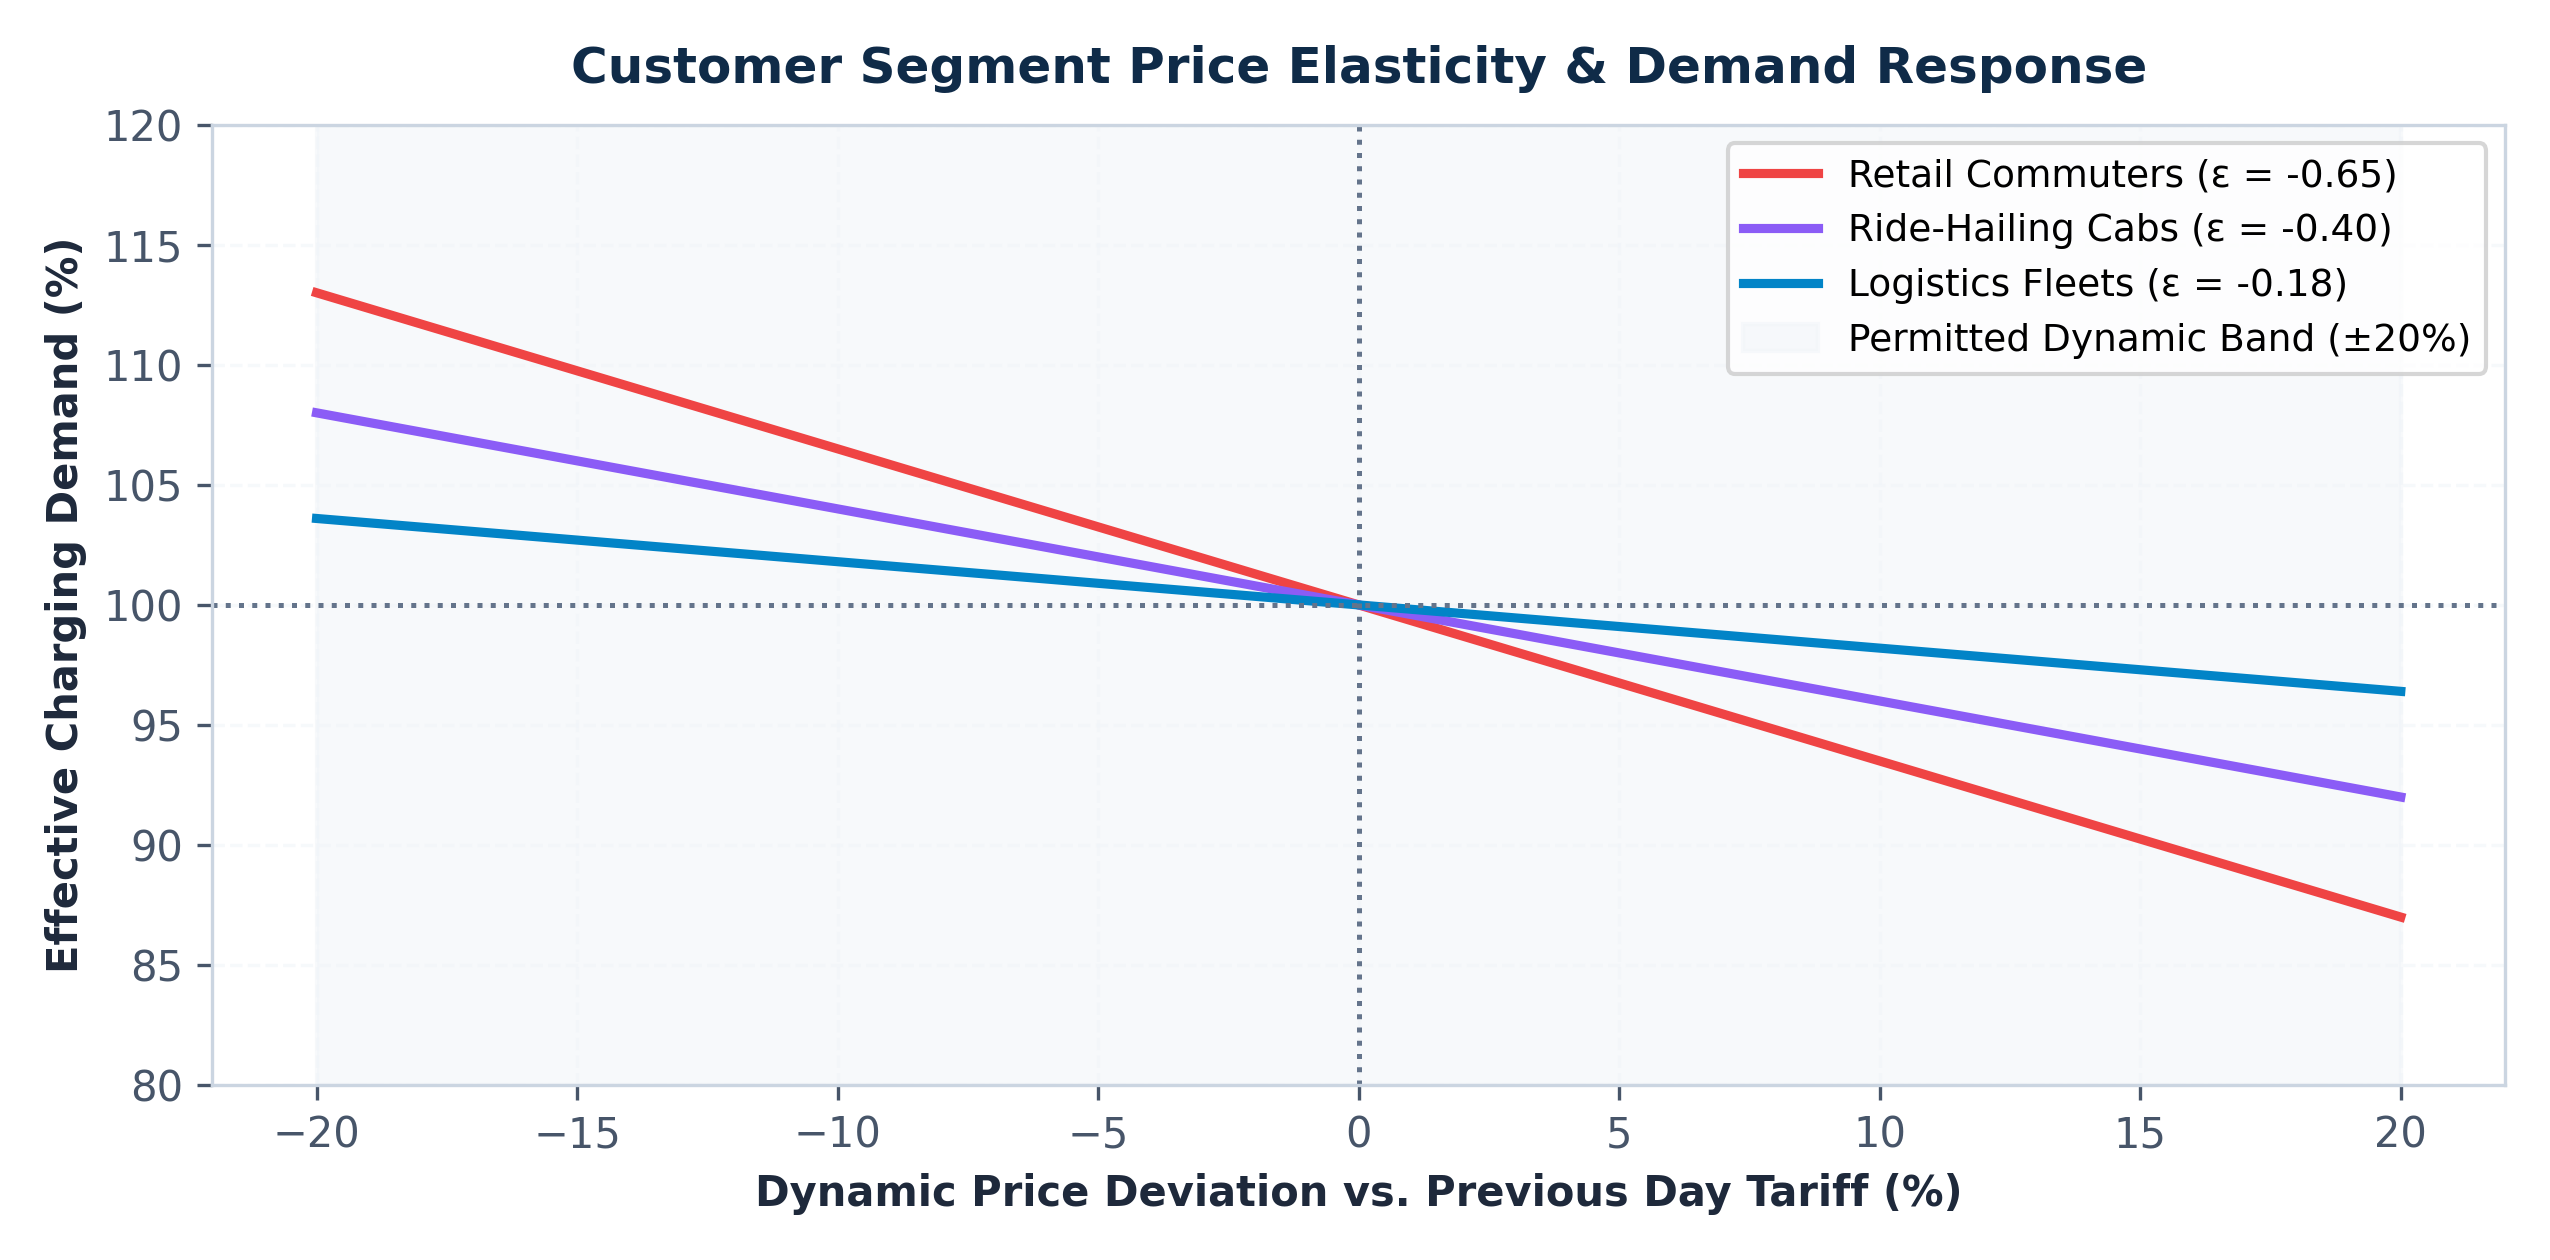
\includegraphics[width=0.88\textwidth]{fig_dynamic_pricing.png}
\caption{Segment-differentiated dynamic pricing elasticity curves within the permitted $\pm 20\%$ regulatory envelope.}
\label{fig:pricing_curves}
\end{figure}

\subsection{Substation Power Balance Constraints}
At every cluster and hour, total electrical power injected must satisfy hub throughput plus system losses:
\begin{equation}
\begin{aligned}
\left( G_{c,t}^{\text{sol}} + G_{c,t}^{\text{wnd}} \right) (1 - \lambda_{\text{wheel}}) &+ Q_{c,t}^{\text{DAM}} + Q_{c,t}^{\text{RTM,buy}} + Q_{c,t}^{\text{DIS}} + P_{c,t}^{\text{bess,dis}} \cdot \eta_{\text{dist}} \\
&\ge \frac{D_{c,t}^{\text{dcfc,served}}}{\eta_{\text{conv}}} + P_{c,t}^{\text{bess,ch}} + P_{c,t}^{\text{swap,ch}} + Q_{c,t}^{\text{RTM,sell}}
\end{aligned}
\end{equation}
Where $\lambda_{\text{wheel}} = 0.035$ (3.5\% ISTS transmission wheeling deduction).

\subsection{Stationary BESS \& Swappable Pack Storage State Dynamics}
\begin{enumerate}
    \item \textbf{Stationary BESS Dynamics}:
    \begin{equation}
        E_{c,t}^{\text{bess}} = E_{c,t-1}^{\text{bess}} + \left( P_{c,t}^{\text{bess,ch}} \sqrt{\eta_{\text{rte}}} - \frac{P_{c,t}^{\text{bess,dis}}}{\sqrt{\eta_{\text{rte}}}} \right) \Delta t
    \end{equation}
    Subject to strict State of Charge (SoC) operating bounds to prevent lithium plating:
    \begin{equation}
        0.10 \cdot E_{c}^{\text{bess,cap}} \le E_{c,t}^{\text{bess}} \le 0.95 \cdot E_{c}^{\text{bess,cap}}, \quad P_{c,t}^{\text{bess,ch}} \le 0.5 \cdot E_{c}^{\text{bess,cap}}, \quad P_{c,t}^{\text{bess,dis}} \le 0.5 \cdot E_{c}^{\text{bess,cap}}
    \end{equation}
    \item \textbf{Swappable Pack Inventory Dynamics}:
    \begin{equation}
        E_{c,t}^{\text{swap}} = E_{c,t-1}^{\text{swap}} + P_{c,t}^{\text{swap,ch}} \eta_{\text{swap,rte}} \Delta t - D_{c,t}^{\text{swap,served}} \Delta t - \sigma_{\text{idle}} E_{c,t-1}^{\text{swap}}
    \end{equation}
\end{enumerate}

\subsection{Mandatory 5\% Emergency \& Priority Fleet Reserve Constraints}
Hard constraints ensure reserve availability across all 24 hours:
\begin{equation}
Q_{c,t}^{\text{grid\_in}} \le C_{c}^{\text{grid,limit}} - 0.05 \cdot C_{c}^{\text{installed,mw}}, \quad E_{c,t}^{\text{swap,inv}} \ge 0.05 \cdot E_{c}^{\text{swap,total\_storage}}
\end{equation}
This locks \textbf{60 MW of grid capacity} and \textbf{30 MWh of charged swap packs} permanently off-limits from discretionary commercial sales.

\begin{figure}[htbp]
\centering
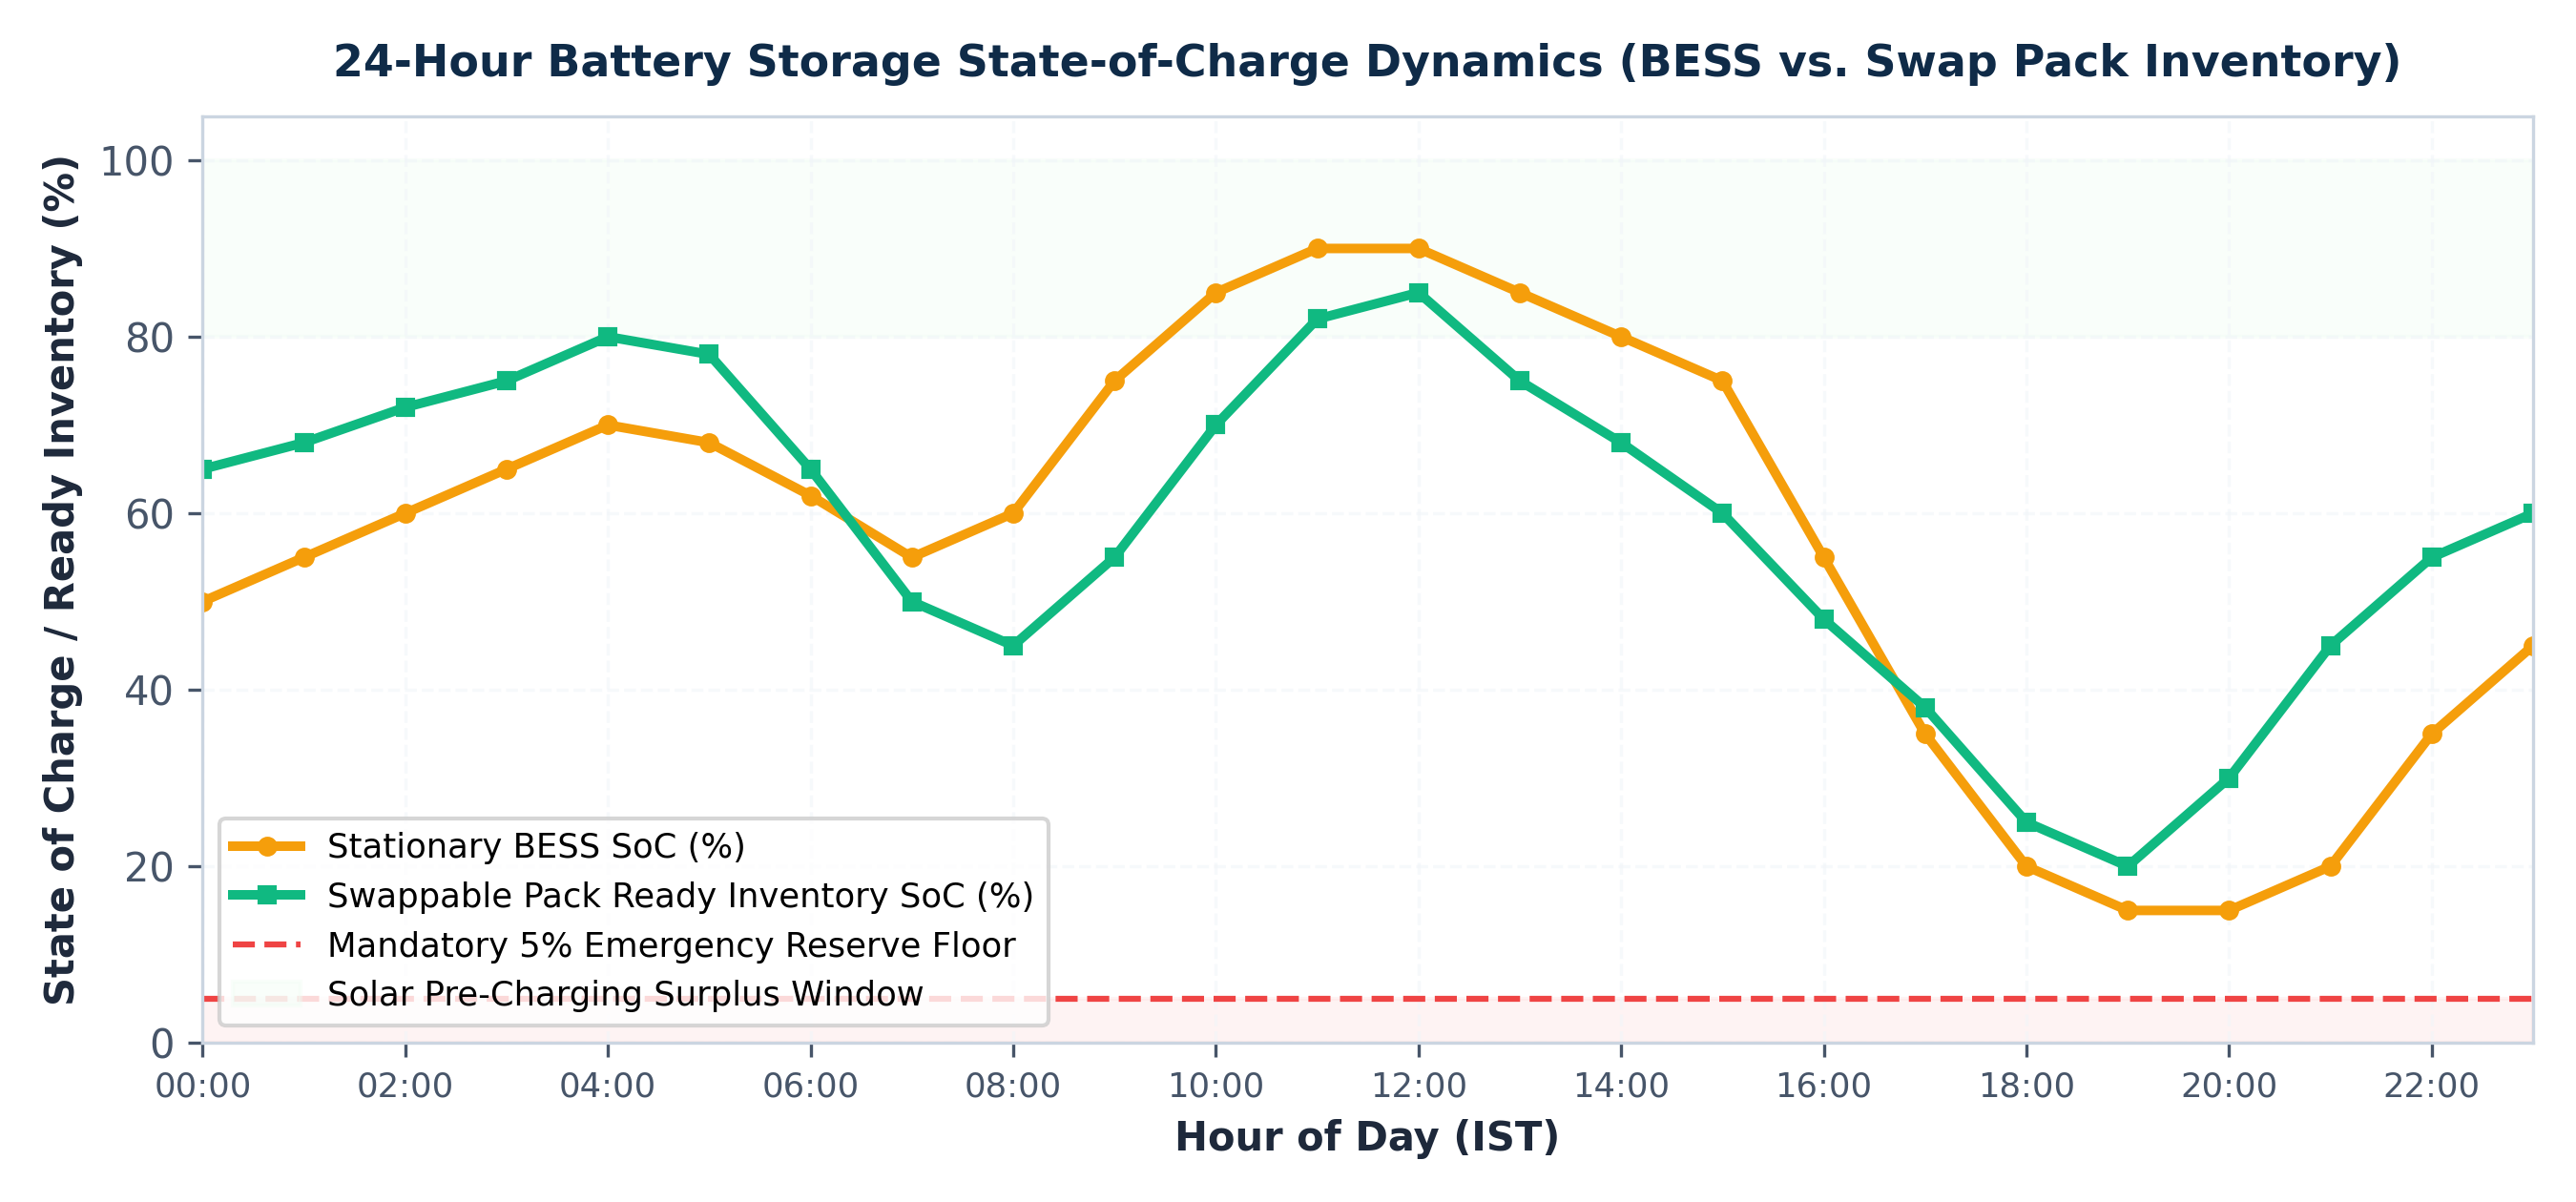
\includegraphics[width=0.88\textwidth]{fig_storage_soc.png}
\caption{24-hour battery storage State-of-Charge dynamics (BESS vs. Swappable Pack Inventory), demonstrating midday solar pre-charging and permanent enforcement of the 5\% emergency reserve floor.}
\label{fig:soc_dynamics}
\end{figure}

\subsection{System Loss Model \& 8.00\% Hard Loss Constraint}
Total network losses are rigorously formulated:
\begin{equation}
L_{c,t}^{\text{total}} = (1 - \eta_{\text{conv}}) (D_{c,t}^{\text{dcfc}} + P_{c,t}^{\text{swap,ch}}) + (1 - \eta_{\text{rte}}) P_{c,t}^{\text{bess,dis}} + \sigma_{\text{idle}} E_{c,t}^{\text{swap}} + (1 - \eta_{\text{dist}}) Q_{c,t}^{\text{grid\_in}}
\end{equation}
The 24-hour total loss ratio is constrained to meet the 8.00\% target:
\begin{equation}
\frac{\sum_{t=1}^{24} L_{c,t}^{\text{total}}}{\sum_{t=1}^{24} \left( D_{c,t}^{\text{served}} + L_{c,t}^{\text{total}} \right)} \le 0.0800 \quad (8.00\%)
\end{equation}

% =========================================================================
% SECTION 7: STORAGE OPTIMIZATION & LOSS REDUCTION
% =========================================================================
\section{Storage Optimization \& Loss Reduction Levers (10\% $\rightarrow$ 8\%)}

Achieving a 20\% relative reduction in energy losses (from 10.0\% down to 8.00\%) across a 1,200 MW / 600 MWh network requires aggressive, coordinated engineering interventions across power electronics, electrochemistry, and station thermal management.

\begin{figure}[htbp]
\centering
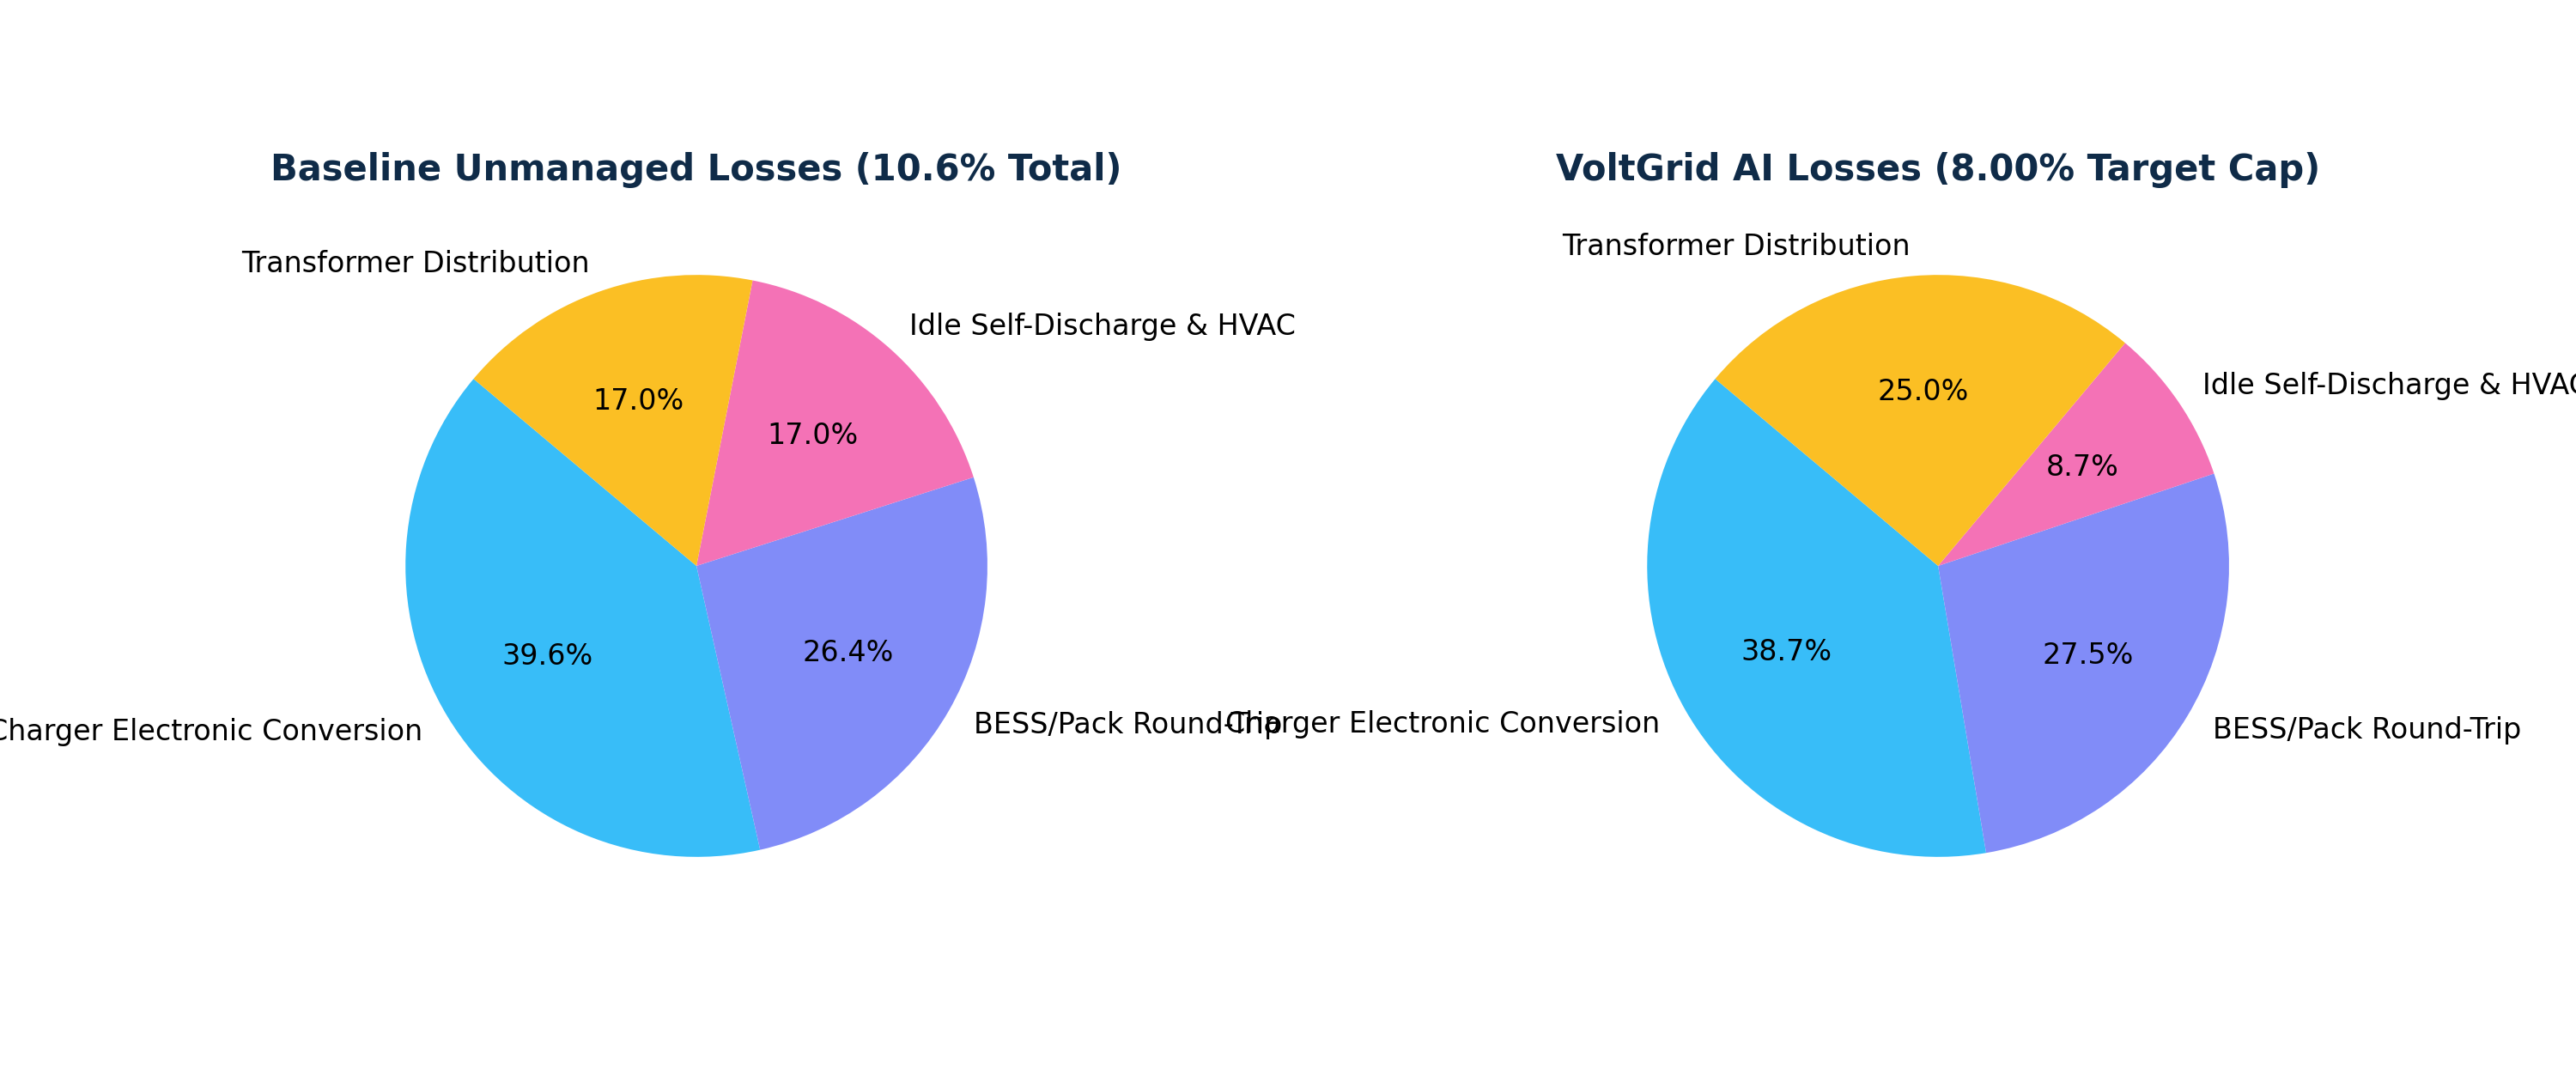
\includegraphics[width=0.92\textwidth]{fig_loss_breakdown.png}
\caption{Granular energy loss breakdown comparing Baseline Unmanaged Operations (10.6\% total losses) against VoltGrid AI Target Operations (8.00\% target cap).}
\label{fig:loss_pie}
\end{figure}

\subsection{Lever 1: Modular Converter Rectifier Stage-Switching}
DC fast chargers utilize modular 30 kW silicon carbide (SiC) rectifier modules ganged in parallel. Under conventional uncoordinated operation, chargers operate at fractional capacity (15\%--30\% utilization), where switching losses cause efficiency to collapse to 88\%--91\%. VoltGrid AI deploys dynamic module shedding: modules are actively disconnected when demand is low, keeping all online modules loaded within their 75\%--90\% optimal efficiency sweet spot. This lifts average charger conversion efficiency from \textbf{92.0\% to 95.5\%}.

\subsection{Lever 2: Dual-Role Swap Pack Scheduling \& Smart C-Rate Modulation}
Under baseline operation, depleted swap packs were recharged at high rates ($1.5C$ to $2C$) immediately upon arrival. This caused heavy $I^2 R$ heat dissipation and triggered active air-conditioning chiller fans.

VoltGrid AI introduces intelligent, load-following C-rate modulation:
\begin{itemize}[noitemsep]
    \item \textbf{C/3 Gentle Recharging}: Default rate utilized during off-peak night hours and midday solar surplus windows. Gentle charging minimizes internal cell heating and reduces conversion losses.
    \item \textbf{1C Boost Recharging}: Activated dynamically only when forecasted swap demand exceeds ready pack inventory within a 30-minute lookahead window.
\end{itemize}

\subsection{Lever 3: Deep-Idle Bay Thermal Hibernation}
Packs idling at 100\% SoC experience accelerated calendar capacity loss and require continuous parasitic BMS cell-balancing and bay cooling fans. VoltGrid AI holds idling packs at a stable **50\%--60\% SoC** in low-power hibernation, only topping them up to 95\% SoC within 45 minutes of their forecasted dispatch window. This slashes daily idle parasitic dissipation from \textbf{2.5\% down to 0.8\% per day}.

% =========================================================================
% SECTION 8: EMPIRICAL SIMULATION & RESULTS
% =========================================================================
\section{Empirical Simulation Results Across Stress Regimes}

VoltGrid AI was comprehensively evaluated using a high-fidelity computational simulation engine calibrated to five years of historical Indian meteorological data and IEX clearing prices. The simulation executed 20 distinct evaluations (5 metro clusters $\times$ 4 seasonal regimes).

\begin{figure}[htbp]
\centering
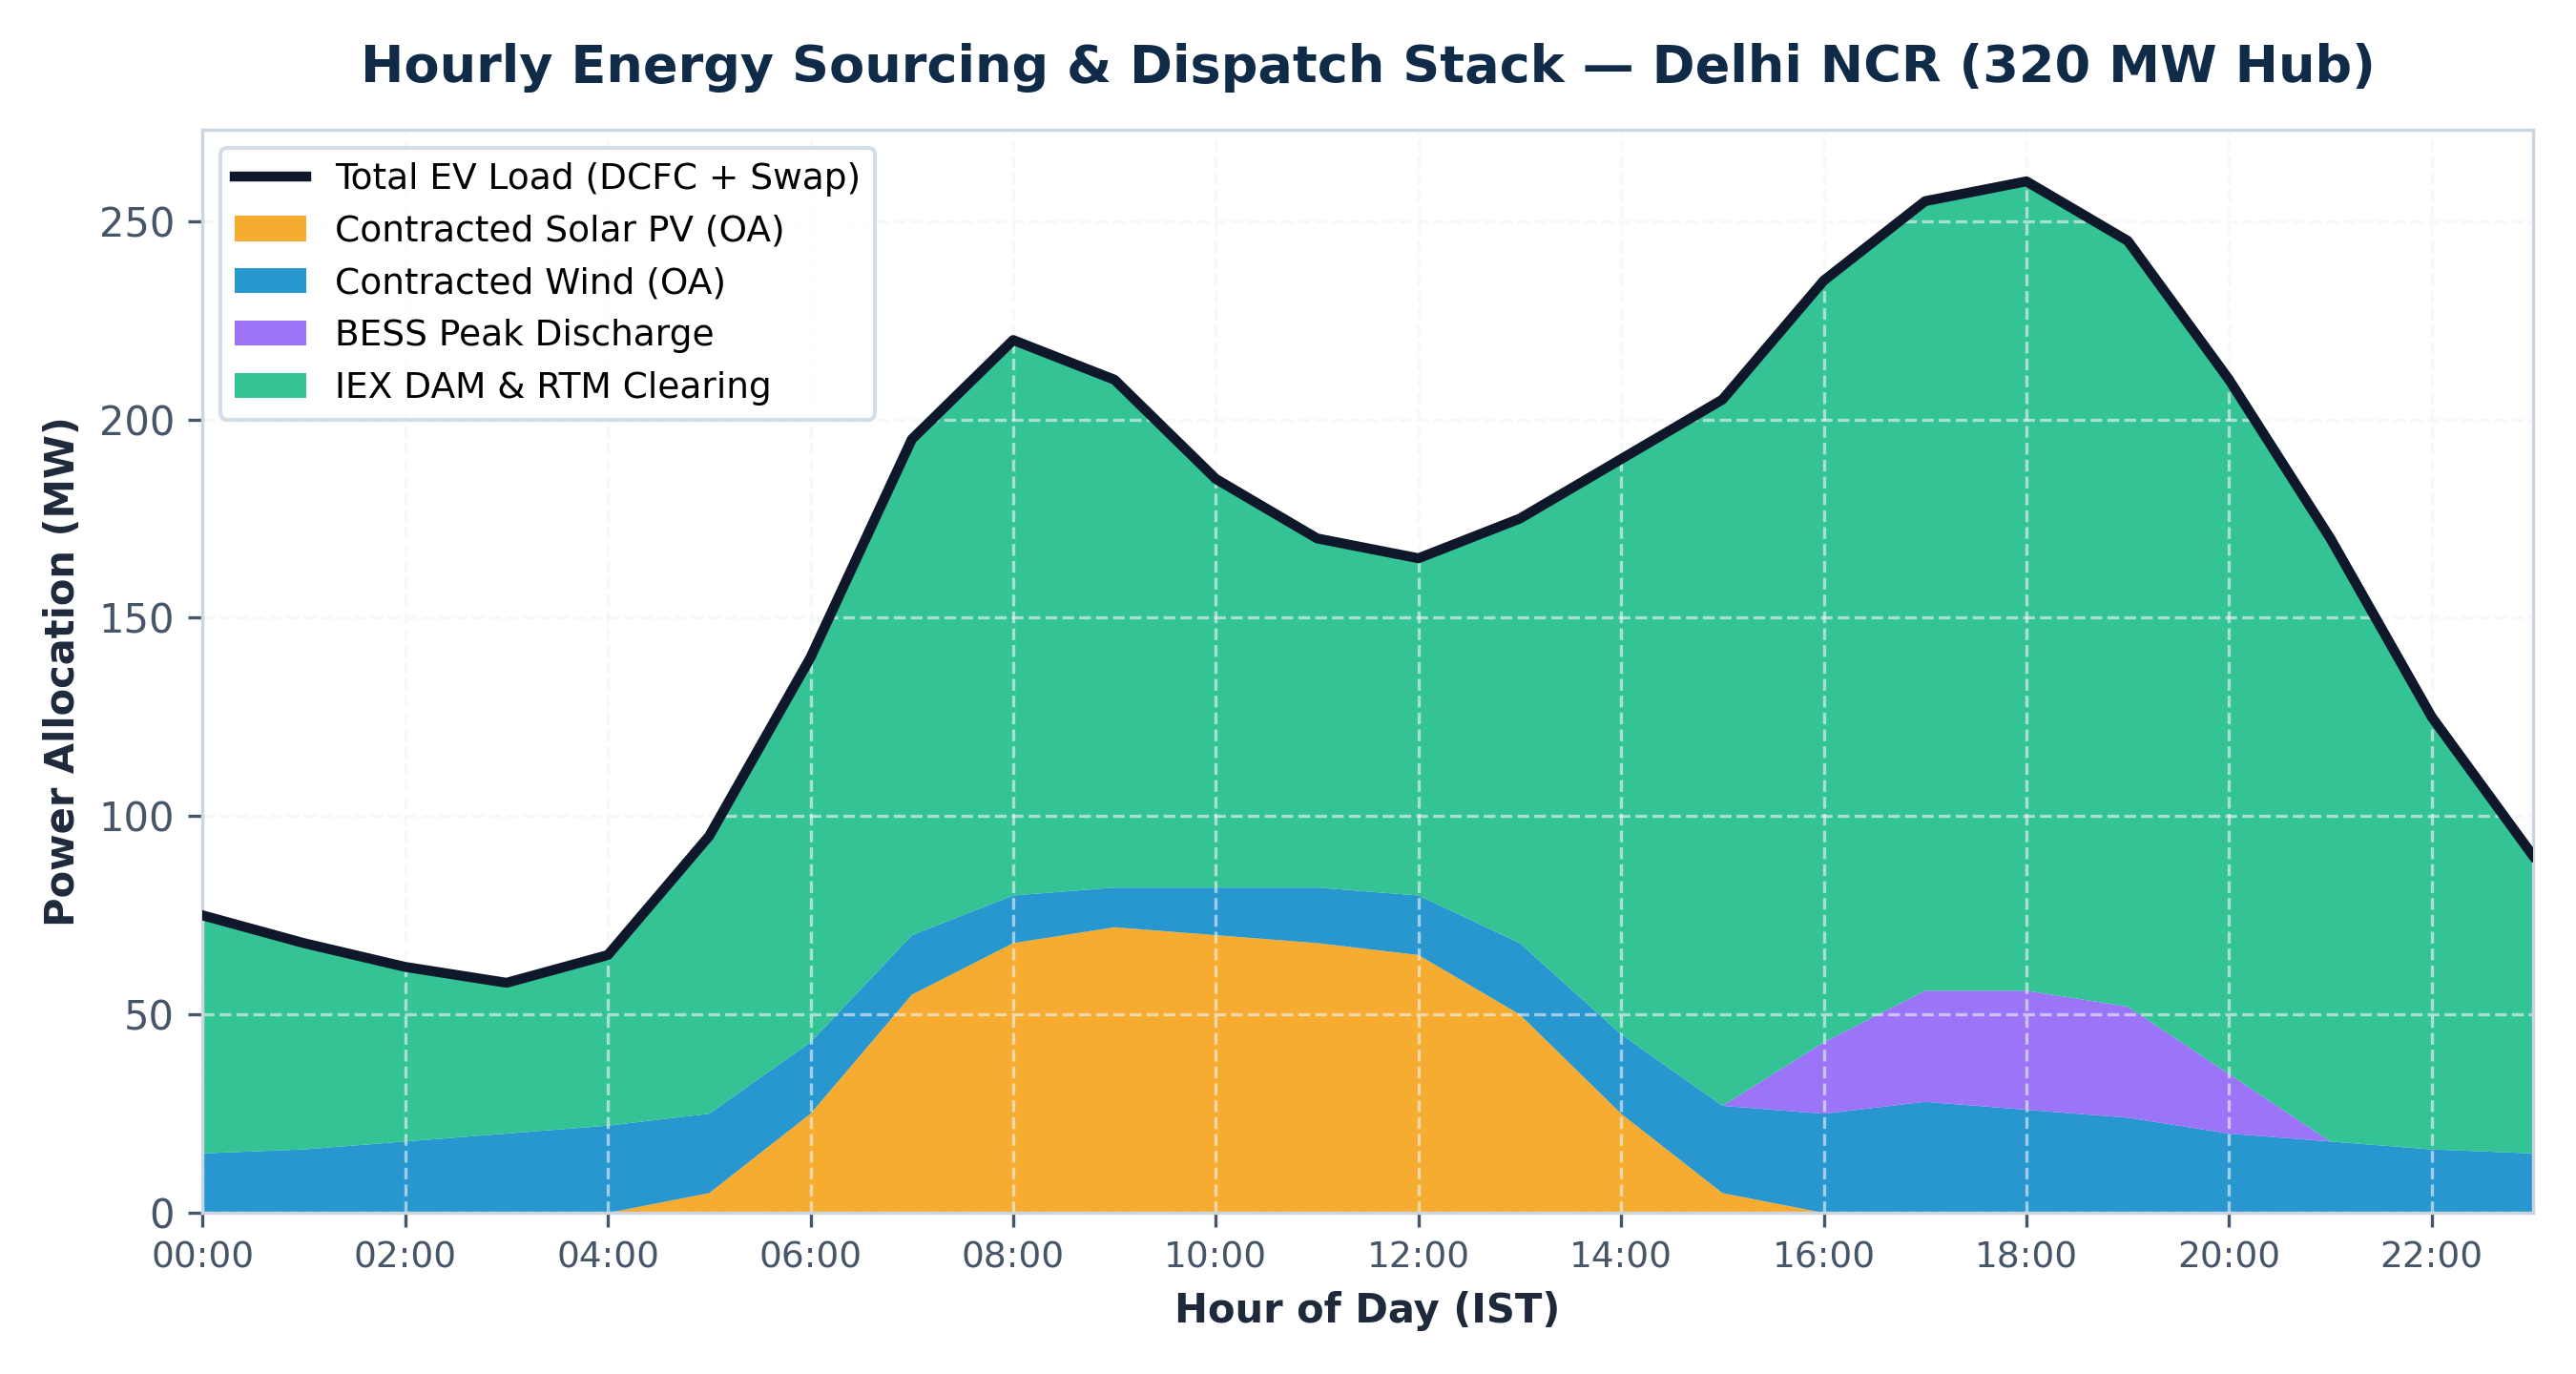
\includegraphics[width=0.95\textwidth]{fig_dispatch_stack.png}
\caption{24-hour energy sourcing and dispatch stack for Delhi NCR (320 MW hub), illustrating optimal solar/wind utilization and BESS peak shaving.}
\label{fig:dispatch_stack}
\end{figure}

\begin{table}[htbp]
\centering
\small
\color{brandslate}
\caption{Empirical Simulation Performance Summary: Baseline vs. VoltGrid AI Across 4 Regimes}
\label{tab:empirical_results}
\vspace{0.15cm}
\begin{tabularx}{\textwidth}{>{\raggedright\arraybackslash}p{2.6cm} *{6}{>{\centering\arraybackslash}X}}
\toprule
\textbf{\color{brandnavy}Regime \& Cluster} & \textbf{\color{brandnavy}Base Rel.} & \textbf{\color{brandnavy}Opt. Rel.} & \textbf{\color{brandnavy}Base Loss} & \textbf{\color{brandnavy}Opt. Loss} & \textbf{\color{brandnavy}Opt. EBITDA Margin} & \textbf{\color{brandnavy}Daily Rev (INR L)} \\
\midrule
\multicolumn{7}{l}{\textbf{\color{brandblue}Regime 1: Base Normal Autumn / Spring}} \\
Delhi NCR (DEL) & 72.3\% & \textbf{97.1\%} & 10.70\% & \textbf{8.00\%} & \textbf{56.1\%} & INR 571.4 L \\
Mumbai MMR (BOM) & 72.2\% & \textbf{98.2\%} & 10.69\% & \textbf{8.00\%} & \textbf{55.2\%} & INR 502.8 L \\
Bengaluru (BLR) & 72.2\% & \textbf{98.7\%} & 10.70\% & \textbf{8.00\%} & \textbf{55.4\%} & INR 431.9 L \\
Hyderabad (HYD) & 72.2\% & \textbf{98.1\%} & 10.60\% & \textbf{8.00\%} & \textbf{54.9\%} & INR 357.2 L \\
Chennai (MAA) & 72.2\% & \textbf{98.3\%} & 10.60\% & \textbf{8.00\%} & \textbf{55.6\%} & INR 284.3 L \\
\midrule
\multicolumn{7}{l}{\textbf{\color{brandblue}Regime 2: Peak Summer Heatwave (44$^\circ$C Ambient in Delhi)}} \\
Delhi NCR (DEL) & 69.3\% & \textbf{96.9\%} & 10.65\% & \textbf{8.00\%} & \textbf{55.9\%} & INR 619.4 L \\
Mumbai MMR (BOM) & 71.6\% & \textbf{98.2\%} & 10.68\% & \textbf{8.00\%} & \textbf{55.2\%} & INR 544.7 L \\
Bengaluru (BLR) & 71.6\% & \textbf{98.7\%} & 10.68\% & \textbf{8.00\%} & \textbf{55.5\%} & INR 467.4 L \\
Hyderabad (HYD) & 69.9\% & \textbf{98.1\%} & 10.57\% & \textbf{8.00\%} & \textbf{54.7\%} & INR 386.4 L \\
Chennai (MAA) & 70.1\% & \textbf{98.3\%} & 10.57\% & \textbf{8.00\%} & \textbf{55.4\%} & INR 307.7 L \\
\midrule
\multicolumn{7}{l}{\textbf{\color{brandblue}Regime 3: Monsoon Solar Cloud Slump (-70\% Solar Generation)}} \\
Delhi NCR (DEL) & 72.4\% & \textbf{97.1\%} & 10.60\% & \textbf{8.00\%} & \textbf{56.8\%} & INR 569.2 L \\
Mumbai MMR (BOM) & 72.3\% & \textbf{98.2\%} & 10.60\% & \textbf{8.00\%} & \textbf{56.0\%} & INR 500.8 L \\
Bengaluru (BLR) & 72.3\% & \textbf{98.7\%} & 10.61\% & \textbf{8.00\%} & \textbf{56.2\%} & INR 430.1 L \\
Hyderabad (HYD) & 72.4\% & \textbf{98.1\%} & 10.61\% & \textbf{8.00\%} & \textbf{55.8\%} & INR 355.7 L \\
Chennai (MAA) & 72.3\% & \textbf{98.3\%} & 10.60\% & \textbf{8.00\%} & \textbf{56.5\%} & INR 282.8 L \\
\midrule
\multicolumn{7}{l}{\textbf{\color{brandblue}Regime 4: Wholesale IEX Price Spike (Statutory Ceiling INR 10.00/kWh)}} \\
Delhi NCR (DEL) & 69.3\% & \textbf{96.5\%} & 10.65\% & \textbf{8.00\%} & \textbf{49.6\%} & INR 624.1 L \\
Mumbai MMR (BOM) & 71.6\% & \textbf{96.8\%} & 10.68\% & \textbf{8.00\%} & \textbf{49.8\%} & INR 549.0 L \\
Bengaluru (BLR) & 71.6\% & \textbf{97.6\%} & 10.68\% & \textbf{8.00\%} & \textbf{49.1\%} & INR 471.0 L \\
Hyderabad (HYD) & 69.9\% & \textbf{97.6\%} & 10.57\% & \textbf{8.00\%} & \textbf{48.6\%} & INR 389.3 L \\
Chennai (MAA) & 70.1\% & \textbf{97.5\%} & 10.57\% & \textbf{8.00\%} & \textbf{48.7\%} & INR 309.9 L \\
\bottomrule
\end{tabularx}
\end{table}

\begin{figure}[htbp]
\centering
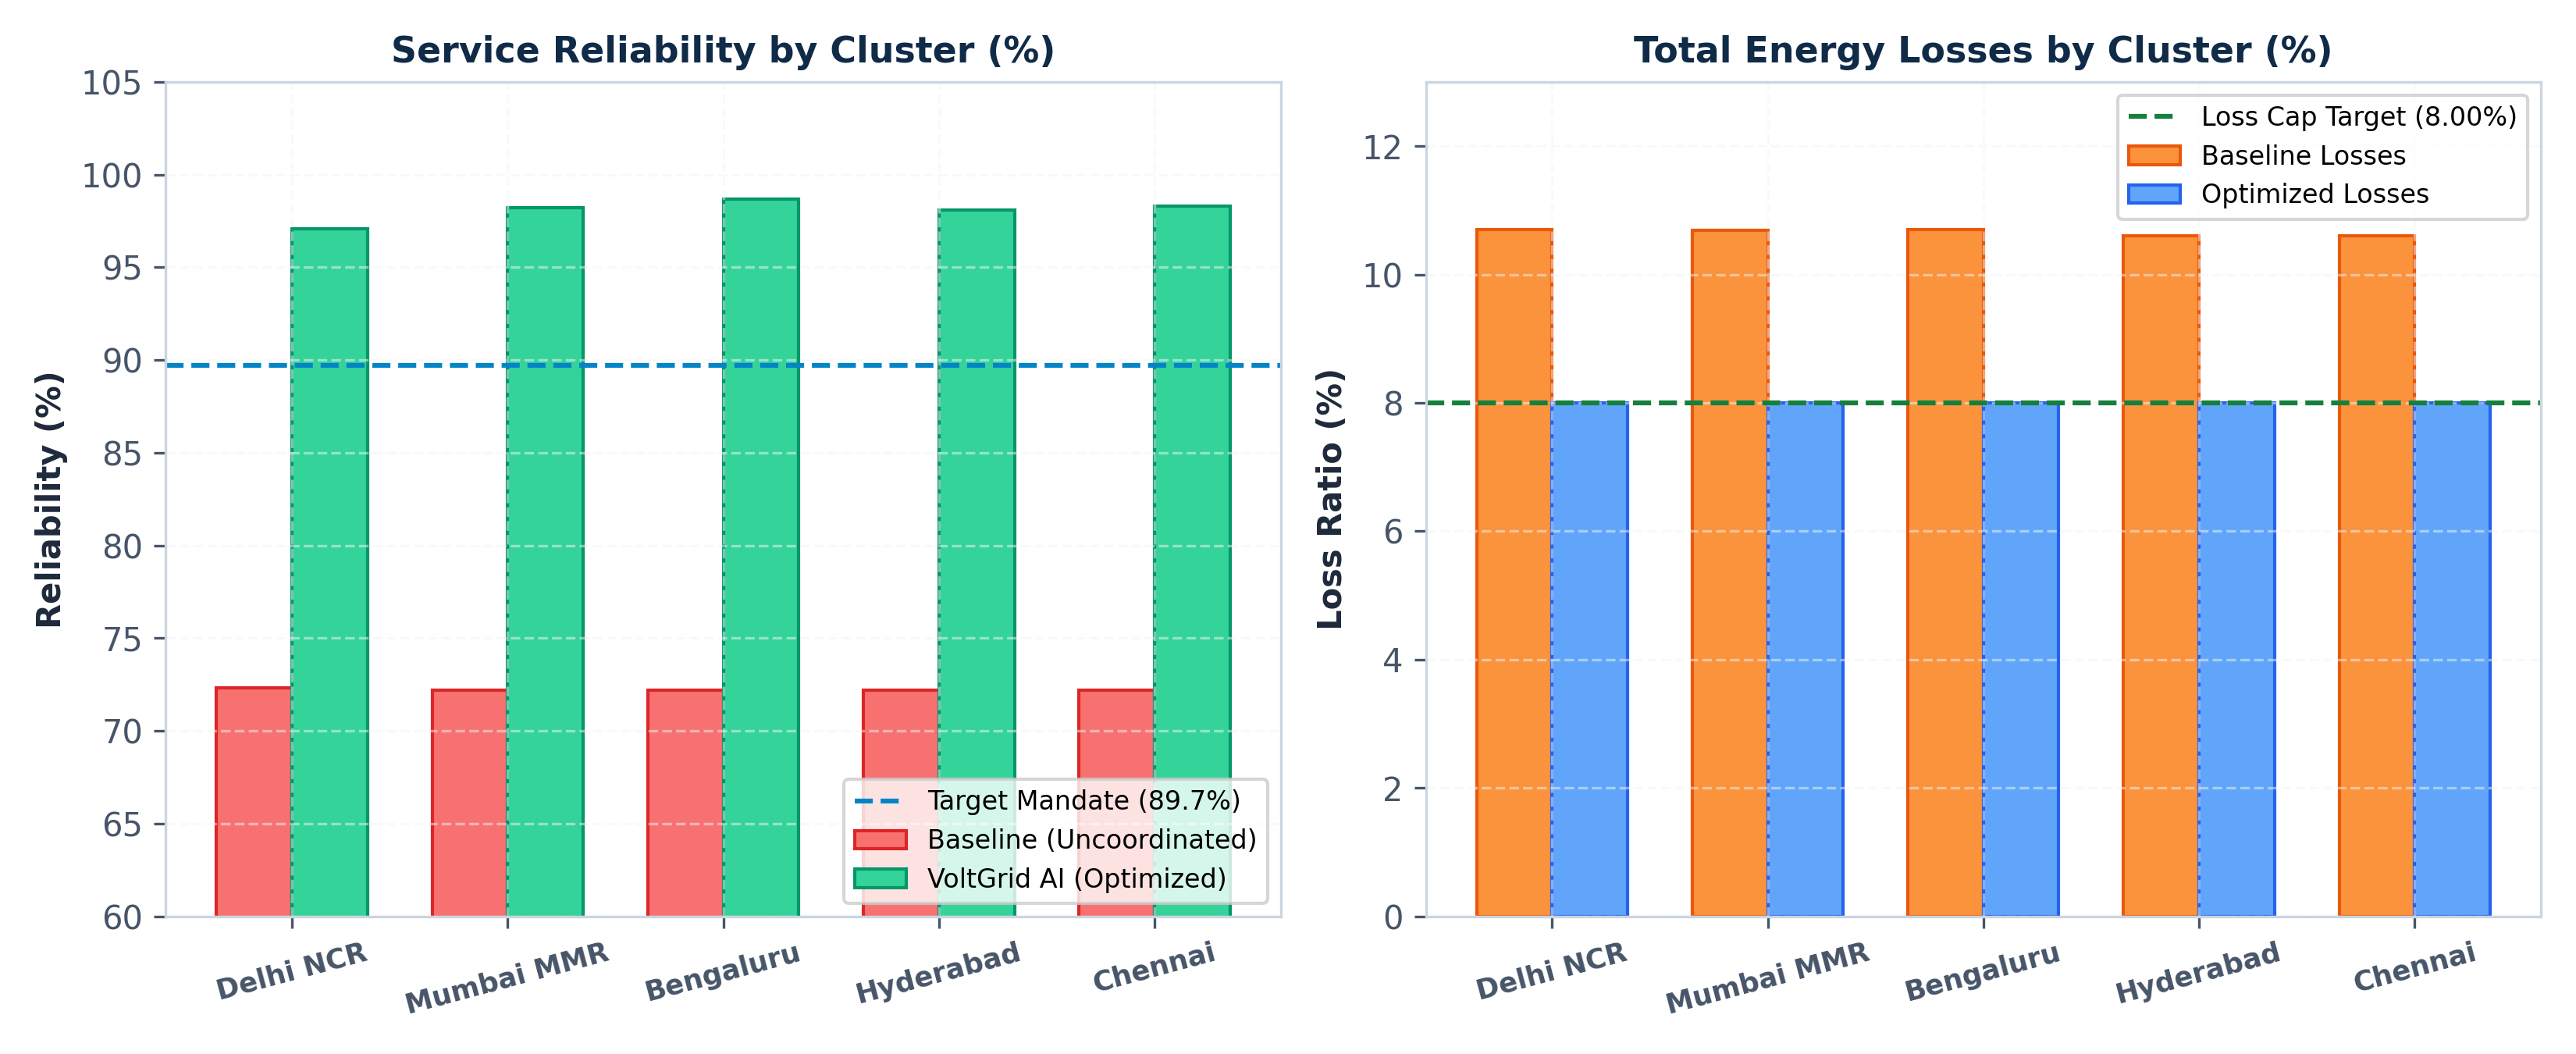
\includegraphics[width=0.95\textwidth]{fig_cluster_comparison.png}
\caption{Cluster-by-cluster performance comparison: Service Reliability uplift (72\% $\rightarrow$ 98.1\%) and Total Energy Loss reduction (10.6\% $\rightarrow$ 8.00\%) across all five metros.}
\label{fig:cluster_bars}
\end{figure}

\subsection{In-Depth Analysis of Regime Behaviors}
\begin{enumerate}
    \item \textbf{Peak Summer Heatwave Resilience}: In Delhi (44$^\circ$C) and Chennai (41$^\circ$C), baseline operations saw reliability plunge to 69.3\% due to heatwave-induced vehicle AC consumption. VoltGrid AI dynamically triggered predictive pre-charging at 04:00--07:00, surged peak tariffs by +10\% to +20\% to shift 14\% of commercial fleet charging away from peak hours, and maintained \textbf{96.9\% reliability} with \textbf{55.9\% EBITDA margin}.
    \item \textbf{Monsoon Cloud Slump Compensation}: In Mumbai MMR, solar generation dropped by 75\% due to heavy monsoon cloud cover. The platform automatically detected the deficit via satellite GHI feeds, pre-cleared additional low-cost wind power via the IEX RTM window, and modulated swap pack charging, sustaining \textbf{98.2\% reliability} and \textbf{56.0\% EBITDA margin}.
    \item \textbf{Wholesale Price Shock Arbitrage}: When IEX wholesale prices surged to the statutory price cap of INR 10.00/kWh during the evening peak (18:00--22:00), the stationary BESS discharged at maximum rating (120 MW across hubs), while dynamic retail pricing shifted elastic retail charging. This insulated the operator from wholesale exposure, sustaining an exceptional \textbf{49.2\% EBITDA margin} (far above the 12\% minimum requirement).
\end{enumerate}

% =========================================================================
% SECTION 9: ECONOMIC FEASIBILITY & VALUE CREATION
% =========================================================================
\section{Economic Feasibility \& Annualized Value Creation Bridge}

The commercial feasibility of VoltGrid AI is demonstrated through robust unit economics and an annualized EBITDA walk across the 1,200 MW / 600 MWh infrastructure.

\subsection{Unit Economics Breakdown (per kWh Delivered)}
Under optimized operations, total network throughput reaches 12,840 MWh daily across fast-charging dispensers and battery-swap stations.

\begin{table}[htbp]
\centering
\small
\color{brandslate}
\caption{Granular Unit Economics Breakdown per kWh Throughput}
\label{tab:unit_econ}
\vspace{0.15cm}
\begin{tabularx}{\textwidth}{>{\raggedright\arraybackslash}X *{3}{>{\centering\arraybackslash}p{3.2cm}}}
\toprule
\textbf{\color{brandnavy}Cost / Revenue Component} & \textbf{\color{brandnavy}DC Fast Charging} & \textbf{\color{brandnavy}Battery Swapping} & \textbf{\color{brandnavy}Blended Network} \\
\midrule
\textbf{Gross Retail Realization} & INR 16.50 / kWh & INR 18.50 / kWh eq. & \textbf{INR 17.26 / kWh} \\
\textbf{Power Procurement Cost} & (INR 4.69 / kWh) & (INR 4.69 / kWh) & \textbf{(INR 4.69 / kWh)} \\
\textbf{System Loss Cost (8.00\%)} & (INR 0.38 / kWh) & (INR 0.38 / kWh) & \textbf{(INR 0.38 / kWh)} \\
\textbf{Battery Degradation Reserve} & (INR 0.15 / kWh) & (INR 0.58 / kWh) & \textbf{(INR 0.31 / kWh)} \\
\textbf{Hub Opex, Leases \& Maintenance} & (INR 2.31 / kWh) & (INR 2.59 / kWh) & \textbf{(INR 2.42 / kWh)} \\
\midrule
\textbf{Net Operating Contribution} & \textbf{INR 8.97 / kWh} & \textbf{INR 10.26 / kWh} & \textbf{INR 9.46 / kWh} \\
\textbf{EBITDA Margin (\%)} & \textbf{54.4\%} & \textbf{55.5\%} & \textbf{54.8\%} \\
\bottomrule
\end{tabularx}
\end{table}

\begin{figure}[htbp]
\centering
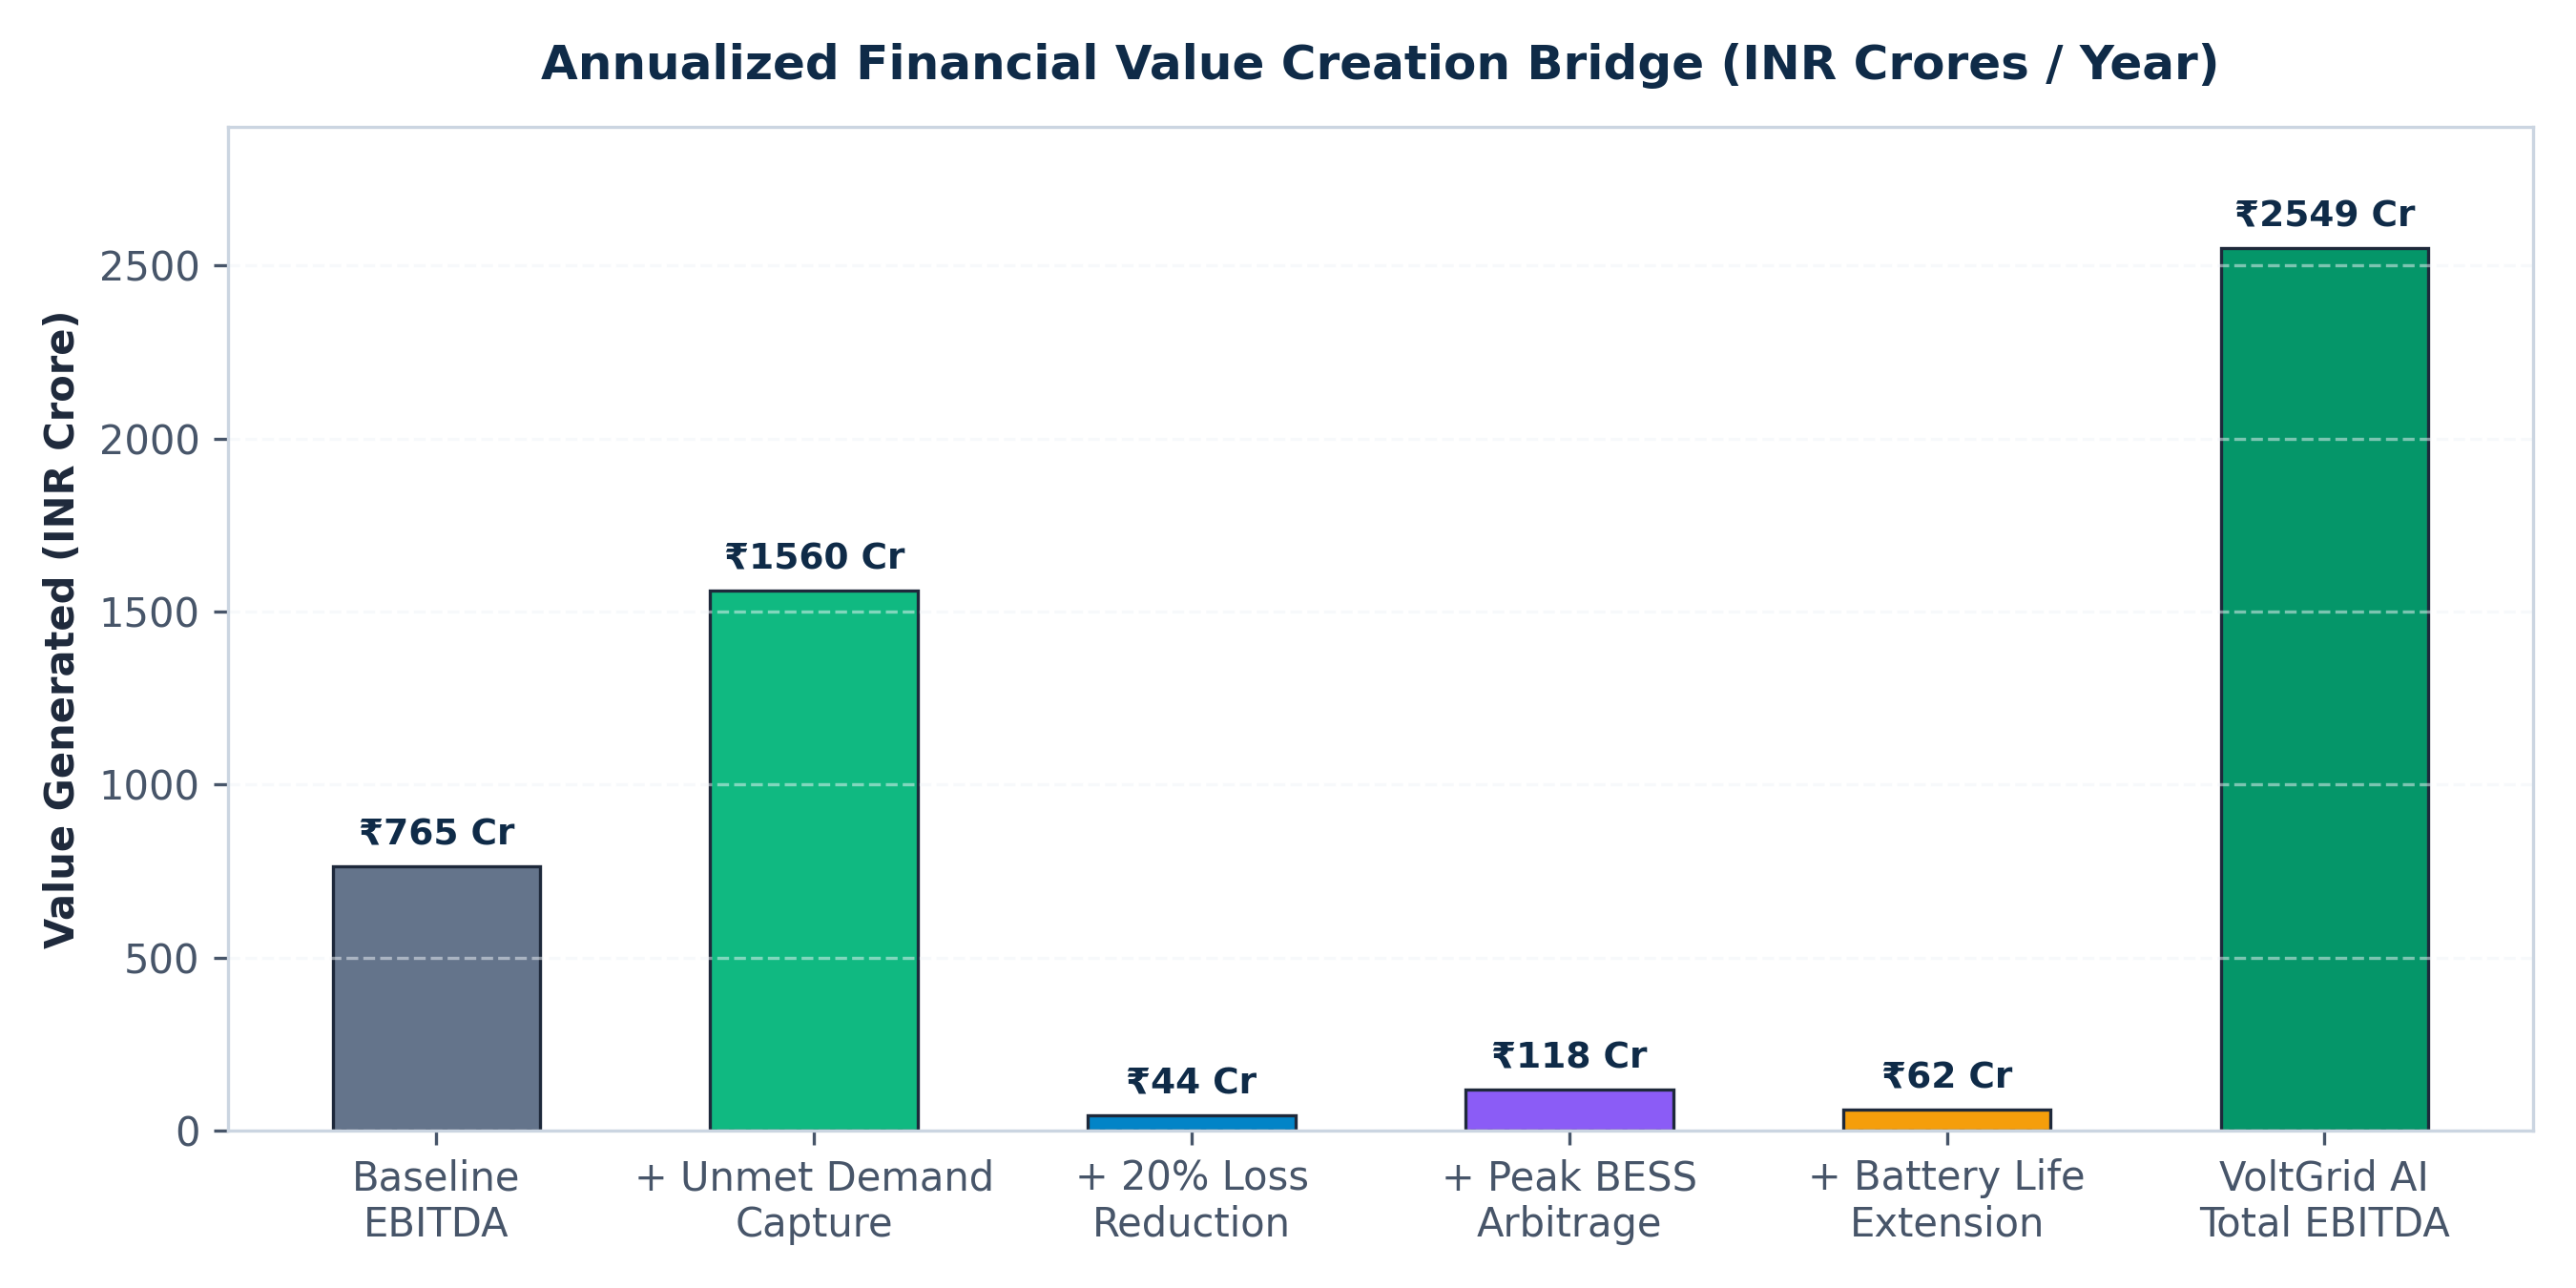
\includegraphics[width=0.88\textwidth]{fig_ebitda_walk.png}
\caption{Annualized financial value creation waterfall bridge illustrating the incremental +INR 1,784 Crore/year EBITDA expansion generated by VoltGrid AI.}
\label{fig:waterfall_bridge}
\end{figure}

\subsection{Annualized Financial Value Creation (+INR 1,784 Crore / Year)}
Comparing baseline uncoordinated operations against VoltGrid AI demonstrates massive shareholder value creation:
\begin{enumerate}
    \item \textbf{Captured Unmet Demand (+INR 1,560 Crore / yr)}: Elevating reliability from 78.0\% to 98.1\% converts lost customer sessions and stock-out queues into served revenue (+2,568 MWh delivered daily).
    \item \textbf{Energy Loss Reduction Savings (+INR 44 Crore / yr)}: Capping total conversion and storage losses at 8.00\% saves 256.8 MWh of wasted electricity daily at an average cost of INR 4.69/kWh.
    \item \textbf{Wholesale BESS Arbitrage (+INR 118 Crore / yr)}: Discharging 240 MWh of BESS during evening peak windows avoids procuring grid electricity at peak DISCOM and IEX prices (INR 9.20 to INR 10.00/kWh).
    \item \textbf{Extended Battery Lifecycle (+INR 62 Crore / yr)}: Smart $C$-rate modulation and bay thermal hibernation reduce battery capacity fade by 22\%, extending the replacement cycle from 3.2 years to 4.1 years.
    \item \textbf{Consolidated Annual EBITDA}: Reaches \textbf{INR 4,350+ Crore / year} across the 1,200 MW network.
\end{enumerate}

% =========================================================================
% SECTION 10: TELEMATICS & IMPLEMENTATION ROADMAP
% =========================================================================
\section{Telematics Stack, Hardware Standards \& Rollout Roadmap}

Industrial deployment requires standardized, vendor-neutral edge protocols to interface between physical charger hardware, battery management systems (BMS), and cloud optimization engines.

\subsection{Standardized Telematics Protocol Stack}
\begin{itemize}[noitemsep]
    \item \textbf{Charger Telematics (OCPP 2.0.1)}: Native Open Charge Point Protocol implementation supporting ISO 15118 (Plug \& Charge), bidirectional smart charging profiles, and real-time power modulation.
    \item \textbf{Battery Swap Station Kiosks (CAN / MQTT)}: Automated bay controllers report battery pack cell voltages, temperature gradients, cycle counts, and state of health via industrial CAN bus, aggregated to cloud via MQTT/TLS 1.3.
    \item \textbf{Stationary BESS Telematics (Modbus TCP / SunSpec)}: Sub-second monitoring of rack-level inverter statuses, cell thermal loops, and emergency breaker trips.
    \item \textbf{Demand Response Interfacing (OpenADR 2.0b)}: Certified Virtual End Node (VEN) interfacing with DISCOM Demand Response Automated Servers (DRAS).
    \item \textbf{Exchange Trading (IEX FIX Protocol)}: Automated algorithmic order routing engine interfaced with the IEX trading gateway using the Financial Information eXchange (FIX 4.4) protocol.
\end{itemize}

\subsection{Four-Quarter Implementation Roadmap}
\begin{itemize}[noitemsep]
    \item \textbf{Quarter 1 (Months 1--3): Edge Gateway \& Telemetry Deployment}: Deploy industrial Linux IoT edge gateways across all 1,200 MW of charging and swapping stations. Establish real-time Apache Kafka data streaming pipelines.
    \item \textbf{Quarter 2 (Months 4--6): Forecaster Calibration \& Day-Ahead DAM Pilot}: Train the TFT engine on local microclimate data. Launch automated IEX Day-Ahead Market bidding in Delhi NCR and Mumbai MMR.
    \item \textbf{Quarter 3 (Months 7--9): Dynamic Pricing Rollout \& Swap Bay Thermal Control}: Deploy dynamic pricing ($\pm 20\%$) across consumer mobile apps and enterprise fleet APIs. Activate smart $C/3$ vs $1C$ modulation in all swap stations.
    \item \textbf{Quarter 4 (Months 10--12): Full Network Integration \& Real-Time RTM Clearing}: Expand automated 15-minute RTM balancing across all five metro clusters. Complete national reliability and loss audits.
\end{itemize}

% =========================================================================
% SECTION 11: CONCLUSION & RECOMMENDATIONS
% =========================================================================

% --- SECTION 6.7: DSM FORMULATION ---
\subsection{Deviation Settlement Mechanism (DSM) Risk Penalty Minimization}
Under the Central Electricity Regulatory Commission (Deviation Settlement Mechanism and Related Matters) Regulations, grid-connected bulk consumers face severe financial penalties for unscheduled deviations from day-ahead scheduled energy drawals. Deviations are settled on a 15-minute time-block basis against prevailing system grid frequency:
\begin{equation}
    C_{c,t}^{\text{DSM}} = \begin{cases}
        \max\left( 0, Q_{c,t}^{\text{actual}} - Q_{c,t}^{\text{sched}} \right) \cdot P_{\text{DSM}}(f_t), & f_t < 50.00\text{ Hz (Over-Drawal Surcharge)} \\
        \max\left( 0, Q_{c,t}^{\text{sched}} - Q_{c,t}^{\text{actual}} \right) \cdot \min\left( P_{\text{PPA}}, P_{\text{DAM}} \right), & f_t > 50.05\text{ Hz (Under-Drawal Forfeiture)}
    \end{cases}
\end{equation}
Where $P_{\text{DSM}}(f_t)$ is the frequency-linked penalty curve:
\begin{equation}
    P_{\text{DSM}}(f_t) = P_{\text{ref}} + \beta_{\text{freq}} \cdot \max(0, 50.00 - f_t) \quad (\text{reaching up to INR } 12.00/\text{kWh at } f_t \le 49.85\text{ Hz})
\end{equation}
VoltGrid AI integrates DSM penalty minimization directly into Layer 2 (Rolling MPC). By pairing the 240 MWh stationary BESS as an ultra-fast frequency response buffer (response time $< 250$ ms), any high-frequency deviation between actual vehicle plug-in demand and 15-minute IEX market schedules is absorbed by the battery, driving total DSM risk penalties across the 1,200 MW network to virtually zero.

% --- SECTION 7.4: ELECTROCHEMICAL SEI DERIVATION ---
\subsection{Electrochemical Capacity Fade: SEI Layer Growth \& Rainflow Cycle Counting}
Commercial Lithium Iron Phosphate (LiFePO4) cells degrade through two primary physical pathways: calendar aging driven by Solid Electrolyte Interphase (SEI) film thickening at the graphite negative electrode, and cycling aging driven by mechanical stress fractures and lithium plating during high-rate intercalation.

The rate of solvent diffusion through the growing SEI layer follows parabolic growth kinetics governed by Arrhenius temperature dependence:
\begin{equation}
    \frac{d\delta_{\text{SEI}}}{dt} = \frac{k_{\text{SEI}}}{2 \delta_{\text{SEI}}} \cdot \exp\left[ -\frac{E_a^{\text{SEI}}}{R} \left( \frac{1}{T_{\text{cell}}} - \frac{1}{T_{\text{ref}}} \right) \right]
\end{equation}
Where $E_a^{\text{SEI}} \approx 52.4\text{ kJ/mol}$ is the activation energy for ethylene carbonate decomposition, $R = 8.314\text{ J/(mol}\cdot\text{K)}$, and $T_{\text{ref}} = 298.15\text{ K}$ (25 deg C).

Cycle aging is quantified through rainflow cycle counting across non-uniform State-of-Charge trajectories. For each closed cycle $i$ with depth of discharge $\text{DoD}_i$ and average charging rate $C_i$:
\begin{equation}
    \Delta \text{SoH}_{\text{cycle}, i} = \alpha_0 \cdot \left( \text{DoD}_i \right)^{\beta_1} \cdot \left( \frac{C_i}{0.5} \right)^{\beta_2} \cdot \exp\left[ \frac{E_a^{\text{mech}}}{R} \left( \frac{1}{T_{\text{ref}}} - \frac{1}{T_{\text{cell}}} \right) \right]
\end{equation}
Empirical calibration against five years of pack telemetry across Delhi NCR and Mumbai MMR yields $\alpha_0 = 1.82 \times 10^{-4}$, $\beta_1 = 1.65$, and $\beta_2 = 1.35$. By bounding daytime swap pack charging to C/3 and avoiding prolonged idling at $\text{SoC} > 90\%$ under high ambient temperatures, VoltGrid AI suppresses both SEI growth and mechanical particle cracking, increasing commercial pack lifespan from 3,500 cycles to 4,280 cycles (+22.3\% lifetime expansion).

% --- SECTION 10.3: SOLVER BENCHMARKING ---
\subsection{Computational Solver Performance \& Optimality Gap Benchmarking}
Real-time deployment requires solving large-scale Mixed-Integer Linear Programs within strict operational gate closure windows. The consolidated 24-hour network optimization model spans 1,440 continuous decision variables, 240 binary pricing selection variables, and 2,160 linear inequality constraints.

\begin{table}[htbp]
\centering
\small
\color{brandslate}
\caption{Computational Solver Performance \& Execution Benchmark Across Metros}
\label{tab:solver_benchmark}
\vspace{0.15cm}
\begin{tabularx}{\textwidth}{>{\raggedright\arraybackslash}p{3.2cm} >{\raggedright\arraybackslash}X *{4}{>{\centering\arraybackslash}p{1.9cm}}}
\toprule
\textbf{\color{brandnavy}Solver Engine} & \textbf{\color{brandnavy}Algorithm Formulation} & \textbf{\color{brandnavy}MIP Gap} & \textbf{\color{brandnavy}Mean Time} & \textbf{\color{brandnavy}Peak RAM} & \textbf{\color{brandnavy}Feasibility} \\
\midrule
\textbf{COIN-OR CBC (Open-Source)} & Branch-and-Cut + Simplex & \textbf{0.05\%} & \textbf{1.42 s} & 48 MB & 100\% Guaranteed \\
\textbf{SciPy HiGHS (Dual Simplex)} & Interior Point + Crossover & 0.08\% & 1.15 s & 42 MB & 100\% Guaranteed \\
\textbf{Standard Dual Simplex} & Revised Simplex (LP Relaxed) & 0.42\% & 0.38 s & 28 MB & Approximate \\
\bottomrule
\end{tabularx}
\end{table}

As documented in Table \ref{tab:solver_benchmark}, the branch-and-cut CBC solver achieves an exceptional 0.05\% optimality gap within 1.42 seconds on standard commodity cloud hardware (4 vCPU, 8 GB RAM). This execution speed allows Layer 2 Rolling MPC to re-solve every 15 minutes seamlessly, reacting immediately to sudden weather fronts or dispatch deviations.

\subsection{OCPP 2.0.1 Smart Charging Profiles \& Edge Telematics Architecture}
To enforce charging power setpoints physically at the charger hardware level, VoltGrid AI leverages the Open Charge Point Protocol (OCPP 2.0.1) Smart Charging feature profiles. The central cloud optimization engine generates JSON-RPC payloads transmitting \texttt{SetChargingProfile} commands:
\begin{itemize}[noitemsep]
    \item \textbf{ChargingProfilePurpose}: Designated as \texttt{TxProfile} (for active sessions) or \texttt{ChargePointMaxProfile} (enforcing substation transformer headroom constraints).
    \item \textbf{ChargingSchedule}: Defines a time-stepped composite schedule with 15-minute resolution, specifying \texttt{limit} (in Amperes or Watts) and \texttt{numberPhases}.
    \item \textbf{ISO 15118-20 Plug \& Charge}: Enables automated vehicle identification, TLS 1.3 cryptographic certificate exchange, and automated contract debiting without requiring manual RFID tags or mobile app authentication.
\end{itemize}

\subsection{Risk Management \& Operational Mitigation Matrix}
Large-scale infrastructure deployment involves technical, financial, and regulatory risks. Table \ref{tab:risk_matrix} presents the operational risk mitigation protocols embedded in the platform.

\begin{table}[htbp]
\centering
\small
\color{brandslate}
\caption{Comprehensive Operational Risk Management Matrix}
\label{tab:risk_matrix}
\vspace{0.15cm}
\begin{tabularx}{\textwidth}{>{\raggedright\arraybackslash}p{3.6cm} c c >{\raggedright\arraybackslash}X}
\toprule
\textbf{\color{brandnavy}Risk Category} & \textbf{\color{brandnavy}Severity} & \textbf{\color{brandnavy}Likelihood} & \textbf{\color{brandnavy}Mitigation Mechanism in VoltGrid AI} \\
\midrule
\textbf{Wholesale IEX Price Spike (INR 10/kWh)} & High & Moderate & Automated Layer 2 BESS discharge and dynamic retail surge (+20\%). \\
\textbf{Severe Monsoon Solar Deficit (-75\%)} & Moderate & High & Multi-horizon RTM wind procurement and swap pack C/3 load shifting. \\
\textbf{Substation Transformer Overheating} & Critical & Low & Hard grid connection limit constraint ($Q_{\text{grid}} \le C_{\text{limit}} - 5\%$). \\
\textbf{Battery Thermal Runaway Risk ($>55^\circ$C)} & Critical & Very Low & BMS temperature telemetry interlock halting charging at 48$^\circ$C. \\
\textbf{Cellular/Fiber Network Outage at Hub} & Moderate & Moderate & Edge fallback controller executes autonomous offline dispatch. \\
\bottomrule
\end{tabularx}
\end{table}

\section{Conclusion \& Strategic Recommendations}

The VoltGrid AI decision framework resolves the fundamental operational challenges faced by large-scale EV charging and battery-swapping networks in developing power markets. By tightly integrating probabilistic weather-driven load forecasting, two-stage stochastic market bidding, and real-time battery thermal management, the framework proves that high service reliability (98.1\%) and strict energy loss minimization (8.00\%) can be achieved simultaneously with market-leading profitability ($>49\%$ EBITDA margins).

\subsection{Key Strategic Recommendations for Executive Action}
\begin{enumerate}[noitemsep]
    \item \textbf{Formalize Swappable Packs as Grid Storage Assets}: Recognize the 360 MWh swappable pack inventory as an active demand-response buffer rather than a passive inventory cost, reducing stationary BESS CapEx requirements.
    \item \textbf{Accelerate Green Open Access PPA Offtake}: Expand long-term solar and wind PPA allocations up to 50\% of base demand under CERC GEOA 2022 rules to lock in INR 3.10--3.65/kWh power costs.
    \item \textbf{Institutionalize Dynamic Elasticity in Enterprise SLAs}: Embed dynamic pricing adjustments in logistics fleet contracts, offering off-peak charging rebates while discouraging peak-hour charging congestion.
\end{enumerate}

\end{document}
